\PassOptionsToPackage{table,svgnames}{xcolor}
\documentclass[11pt,a4paper]{report}

%%------------------------------- PREAMBLE ------------------------------------

%% 1. Language & Encoding (Quan trọng: Load trước để tránh lỗi font)
\usepackage[utf8]{inputenc}       
\usepackage[T1,T5]{fontenc}       % T5 cho tiếng Việt
\usepackage[english, vietnamese]{babel} % Hỗ trợ cả 2 ngôn ngữ

%% 2. Fonts & Math
\usepackage{newtxtext,newtxmath}  % Font giống report-pi (Times style)
\usepackage{amsmath}              
\usepackage{setspace}             

%% 3. Graphics & Colors
\usepackage{graphicx}             
\usepackage{caption}              
\usepackage{subcaption}           
\usepackage{float}                
\usepackage[normalem]{ulem}       

%% --- Định nghĩa màu chủ đạo của Template (QUAN TRỌNG) ---
\usepackage{color}
% Màu nâu đỏ đặc trưng của template report-pi
\definecolor{engineering}{rgb}{0.549,0.176,0.098} 
\definecolor{cloudwhite}{cmyk}{0,0,0,0.025}

%% 4. Tables & Lists
\usepackage{longtable}            
\usepackage{multirow}             
\usepackage{booktabs}
\usepackage{lipsum}               
\usepackage{csquotes}             

%% 5. Bibliography
\usepackage[backend=biber,authordate]{biblatex-chicago}
\addbibresource{bibliography.bib}

%% 6. Advanced Packages (Code, Box, Diagram)
\usepackage{pgfgantt}             
\usepackage{todonotes}            
\setlength{\marginparwidth}{2cm}

% Tcolorbox (Giữ lại từ main.tex của bạn)
\usepackage{tcolorbox}
\tcbuselibrary{breakable, skins, listings}
\usepackage{eurosym} 

% Listings (Code block style giống report-pi)
\usepackage{listings}
\lstset{ 
 language=C,          
 basicstyle=\footnotesize\ttfamily,
 keywordstyle=\bfseries,
 numbers=left,                      
 numberstyle=\scriptsize\texttt,    
 stepnumber=1,                      
 numbersep=8pt,                     
 frame=tb,
 float=htb,
 aboveskip=8mm,
 belowskip=4mm,
 backgroundcolor=\color{cloudwhite},
 showspaces=false,                  
 showstringspaces=false,            
 showtabs=false,                
 tabsize=2,                         
 captionpos=t,                      
 belowcaptionskip=12pt,             
 breaklines=true,         
 breakatwhitespace=false,           
 escapeinside={\%*}{*)},            
 morekeywords={*,var,template,new}  
}

%% 7. Layout & Headers (Giống report-pi)
\usepackage[a4paper,left=25mm,right=25mm,top=25mm,bottom=25mm,headheight=6mm,footskip=12mm]{geometry}
\setlength{\parindent}{0em}
\setlength{\parskip}{1ex}

\usepackage{lastpage}
\usepackage{fancyhdr}
\fancyhf{}                            % Xóa header/footer mặc định
% Header bên phải: Tên đồ án, Tên tác giả
\rhead{\small{\emph{\projtitle, \projauthor}}} 
% Footer bên phải: Số trang / Tổng số trang
\rfoot{\small{\thepage\ / \pageref{LastPage}}}
\pagestyle{fancy}                     % Kích hoạt style
\renewcommand{\headrulewidth}{0.4pt}
\renewcommand{\footrulewidth}{0.4pt}

%% 8. Hyperlinks (Tạo màu cho link giống template)
\usepackage{hyperref}
\hypersetup{
    plainpages=false, 
    pdfpagelayout=SinglePage,
    bookmarksopen=false,
    bookmarksnumbered=true,
    breaklinks=true,
    linktocpage,
    colorlinks=true,         % Bật màu
    linkcolor=engineering,   % Màu nâu đỏ cho mục lục/link nội bộ
    urlcolor=engineering,    % Màu nâu đỏ cho URL
    filecolor=engineering,
    citecolor=engineering,   % Màu nâu đỏ cho trích dẫn
    allcolors=engineering
}

%% 9. Macros (Các biến thông tin - Cần cập nhật theo nội dung của bạn)
\graphicspath{{figures/}}

\newcommand{\school}{Institut National des Sciences Appliquées de Toulouse}
\newcommand{\degree}{Bachelor's Degree in Computer Science and Engineering}
\newcommand{\projtitle}{Optimizing and Adapting Language Models for Domain-Specific Task}
\newcommand{\subtitle}{End-of-studies Apprenticeship Report}
\newcommand{\projauthor}{Minh Duy Nguyen}
\newcommand{\supervisor}{Milad Mozafari (Torus AI), David Bertoin (INSA Toulouse)}
\newcommand{\tutor}{David Bertoin}

% Các định nghĩa khác
\newcommand{\windspt}{\textsf{WindsPT\/}}
\newcommand{\windscannerpt}{\emph{Windscanner.PT\/}}
\newcommand{\class}[1]{{\normalfont\sffamily #1\/}}
\newcommand{\svg}{\class{SVG}}

% Environment cho Box thông tin (Màu xanh) giống report-pi
\newenvironment{info}[1]{\vspace*{6mm}\color{blue}[ \textbf{INFO:} \begin{em} #1}
                        {\vspace*{3mm}\end{em} ]}
\newenvironment{infoopt}[1]{\vspace*{6mm}\color{blue}[ \textbf{INFO (optional element):} \begin{em} #1}
                        {\vspace*{3mm}\end{em} ]}

% Environment cho HTML Code (Giữ lại từ main.tex của bạn)
\newtcblisting{htmlcode}{
    arc=2pt, outer arc=2pt, boxrule=0.5pt,
    colback=gray!5, colframe=gray!60!black,
    listing only, top=0pt, bottom=0pt, middle=1pt, boxsep=3pt,
    listing options={
        basicstyle=\tiny\ttfamily, numbers=none, breaklines=true,
        language=HTML, tabsize=2, extendedchars=true,
        literate={€}{{\euro}}1 {é}{{\'e}}1 {â}{{\^a}}1 {à}{{\`a}}1 {ô}{{\^o}}1 {ê}{{\^e}}1,
    },
    title=\textbf{Parsed HTML Output}, fonttitle=\small\sffamily,
    colbacktitle=gray!20!white, coltitle=black, enhanced, width=\textwidth, right=5mm,
}
%%------------------------------- document-------------------------------------

\begin{document}

%% preamble page numbers with roman numerals
\pagenumbering{roman}\setcounter{page}{1}

%%------------------------------- cover page ----------------------------------

\begin{titlepage}
\center

\vspace{-15mm}
{\large \textbf{\textsc{\school}}}\\

\vfill

{\Large \textbf{\projtitle}}\\[8mm]
{\large \textbf{\subtitle}}\\[28mm]

{\Large \textbf{\projauthor}}\\

\vfill

\includegraphics[width=52mm]{figures/logo-INSA.png}
\includegraphics[width=52mm]{figures/logo-N7.png}

\vfill

{\large \degree}\\[8mm]
% {\large \textbf{Tutor na U.Porto}: \tutor}\\[2mm]
{\large \textbf{Supervised by}: \supervisor}\\[8mm]

%\renewcommand{\today}{15 de dezembro de 2023}
\today

\end{titlepage}

%%------------------------------- chapter ------------------------------------
\pagenumbering{arabic}
\chapter{Introduction}

\section{General Context}

\subsection{Sự phát triển của Mô hình Ngôn ngữ Lớn}

Trong thập kỷ qua, lĩnh vực Trí tuệ nhân tạo (Artificial Intelligence - AI) và Xử lý ngôn ngữ tự nhiên (Natural Language Processing - NLP) đã chứng kiến những bước tiến đột phá, đặc biệt kể từ sự ra đời của kiến trúc Transformer [Vaswani et al., 2017]. Các Mô hình Ngôn ngữ Lớn (Large Language Models - LLMs) như GPT-4 [OpenAI, 2023], Claude 3 [Anthropic, 2024], Gemini 1.5 [Google, 2024], cùng các mô hình mã nguồn mở như Llama 3 [Meta, 2024] và Qwen 2.5 [Alibaba, 2024] đã chứng minh khả năng vượt trội trong việc hiểu ngữ cảnh, sinh văn bản và thực hiện suy luận logic trên đa dạng tác vụ.

Theo báo cáo của McKinsey Global Institute (2024), thị trường AI tạo sinh (Generative AI) dự kiến đạt giá trị 4.4 nghìn tỷ USD vào năm 2030. Tuy nhiên, một khảo sát từ Gartner (2024) chỉ ra rằng **67\% doanh nghiệp** gặp khó khăn trong việc triển khai LLMs cho các tác vụ chuyên biệt do các hạn chế về độ chính xác và chi phí vận hành.

\subsection{Khoảng cách giữa Nghiên cứu và Ứng dụng Công nghiệp}

Việc chuyển giao các mô hình ngôn ngữ từ môi trường nghiên cứu sang ứng dụng thực tiễn trong công nghiệp (Industrial Deployment) đang đối mặt với những thách thức đáng kể. Mặc dù các mô hình nền tảng (Foundation Models) sở hữu lượng tri thức tổng quát khổng lồ, chúng thường gặp hai nhóm hạn chế nghiêm trọng khi giải quyết các bài toán chuyên biệt (Domain-specific tasks):

**Khoảng cách về Tri thức (Knowledge Gap):**

Trong các lĩnh vực quan trọng như y tế, tài chính và bảo hiểm, thông tin thường nằm trong các tài liệu phức tạp (báo cáo tài chính, bảng danh mục kỹ thuật y tế) và thay đổi liên tục. Các LLMs đối mặt với ba vấn đề chính:

- **Dữ liệu tĩnh (Static Knowledge):** Tri thức của mô hình bị giới hạn bởi thời điểm huấn luyện (knowledge cutoff), không thể cập nhật thông tin mới mà không cần huấn luyện lại [Lewis et al., 2020].
- **Thiếu dữ liệu nội bộ (Private Data Inaccessibility):** Mô hình không thể truy cập các tài liệu bảo mật của tổ chức như hợp đồng, quy trình nội bộ, hay hồ sơ bệnh nhân.
- **Hiện tượng ảo giác (Hallucination):** LLMs có xu hướng sinh ra thông tin sai lệch một cách tự tin [Ji et al., 2023], điều không thể chấp nhận trong các quyết định y khoa hay tài chính, nơi yêu cầu độ chính xác gần như tuyệt đối.

**Khoảng cách về Hiệu quả và Hành vi (Efficiency \& Behavior Gap):**

Đối với các tác vụ yêu cầu mô hình tuân thủ một kịch bản hành vi cụ thể, một phong cách ngôn ngữ đặc thù (ví dụ: tư vấn viên tâm lý, chuyên gia phân tích), hoặc triển khai trên hạ tầng phần cứng giới hạn, việc sử dụng các mô hình khổng lồ (hàng trăm tỷ tham số) là không tối ưu về chi phí và độ trễ. Theo Hoffmann et al. (2022), chi phí inference của GPT-4 có thể lên tới **\$0.06/1000 tokens**, khiến việc triển khai quy mô lớn trở nên không khả thi cho nhiều doanh nghiệp vừa và nhỏ.

\subsection{Động lực nghiên cứu}

Xuất phát từ thực tế trên, luận văn này tập trung nghiên cứu và triển khai các kỹ thuật tiên tiến nhằm **tối ưu hóa và thích ứng Language Models cho các miền dữ liệu đặc thù**, với hai hướng tiếp cận chính:

1. Retrieval-Augmented Generation (RAG): Tích hợp tri thức bên ngoài để giải quyết Knowledge Gap.

2. Parameter-Efficient Fine-Tuning (PEFT): Thích ứng hành vi mô hình để giải quyết Behavior Gap.

\section{Internship Environment}

This master's thesis was completed at Torus AI, a technology company with the mission "Intelligence for Life," specializing in providing advanced AI solutions to improve quality of life and business efficiency.

I worked in the Research and Development Team (R\&D Team - Torus Lab) as a Machine Learning Engineer Alternant. At Torus AI, the R\&D department acts as a bridge between the latest academic research (State-of-the-Art) and commercial products. The team's main task is to continuously explore emerging Generative AI technologies, assess their feasibility, and build functional prototypes (PoCs) to verify their effectiveness before integration into the main product system.

The R\&D work environment demands flexible thinking: not just using existing APIs, but delving into customizing architecture, optimizing data processing pipelines, and quantitatively evaluating technical solutions.

Vai trò của tôi trong bộ phận R\&D bao gồm:

- Khảo sát các công nghệ Generative AI mới nổi

- Đánh giá tính khả thi và xây dựng các bản mẫu chức năng (Functional Prototypes/PoC)

- Tích hợp các giải pháp vào hệ thống sản phẩm

Tài nguyên được cung cấp:

- Hạ tầng GPU: NVIDIA RTX 3090 (24GB).

- Dữ liệu doanh nghiệp thực tế: Tài liệu y tế (CCAM, NGAP), báo cáo tài chính bảo hiểm

- API access: OpenAI GPT-4, Google Gemini, Qwen API

\section{Problem Statement}

During our work in the R\&D department, we identified two core problems that needed to be addressed when applying GenAI in practice, corresponding to two main technical approaches:

\textbf{Problem 1: Integration of External Knowledge from Complex Unstructured Data}

Partner businesses (such as insurance companies, healthcare facilities) possess large amounts of data in the form of PDF documents containing text, tables, and images. Traditional RAG (Retrieval-Augmented Generation) methods based on plain text (text-only) fail to understand the semantics of complex tables or visual information.
The question is: How to build a Multimodal RAG pipeline capable of accurately parsing, indexing, and retrievaling information from these mixed documents to support decision-making (e.g., medical refund code lookup, financial data analysis)?

\textbf{Problem 2: Behavioral Adaptation and Resource Optimization for Small Models (Behavioral Adaptation \& Efficiency)}

For applications requiring high interactivity, counseling, or entertainment (such as psychological counseling chatbots or Tarot Readers), the requirement is not only for information accuracy but also for consistency in tone and style and rule-based reasoning. Using large models (like GPT-4) via APIs is both costly to operate and difficult to fully control behavior.
The question is: Is it possible to fine-tune small language models (such as Qwen, Llama < 7B parameters) using parameter optimization techniques (PEFT/LoRA) and quantization so that they achieve inference capabilities and writing styles comparable to large models, but can be run locally at low cost?

\section{Phát biểu vấn đề nghiên cứu (Problem Statement)}

\subsection{Các câu hỏi nghiên cứu (Research Questions)}

Trong quá trình làm việc tại bộ phận R\&D, chúng tôi đã xác định hai nhóm vấn đề cốt lõi cần giải quyết khi áp dụng Generative AI vào thực tế, được hình thức hóa thành các câu hỏi nghiên cứu sau:


RQ1 (Research Question 1): Làm thế nào để xây dựng một pipeline Multimodal RAG có khả năng phân tích cú pháp (parsing), lập chỉ mục (indexing) và truy xuất (retrieval) chính xác thông tin từ các tài liệu hỗn hợp (văn bản, bảng biểu, hình ảnh) để hỗ trợ ra quyết định trong lĩnh vực y tế và tài chính?

Bối cảnh: Các doanh nghiệp đối tác sở hữu lượng lớn dữ liệu dưới dạng tài liệu PDF chứa văn bản, bảng biểu (tables) và hình ảnh (charts/images). Các phương pháp RAG truyền thống dựa trên văn bản thuần túy (text-only) thất bại trong việc hiểu ngữ nghĩa của bảng biểu phức tạp hoặc thông tin thị giác.


RQ2 (Research Question 2): Liệu có thể tinh chỉnh (Fine-tuning) các mô hình ngôn ngữ nhỏ (Small Language Models - SLMs, < 7B tham số) bằng các kỹ thuật tối ưu tham số (PEFT/LoRA) và lượng tử hóa (Quantization) để đạt được khả năng suy luận và văn phong tương đương các mô hình lớn, nhưng có thể chạy cục bộ với chi phí thấp?

Bối cảnh: Đối với các ứng dụng yêu cầu tính tương tác cao, mang tính chất tư vấn (như chatbot tư vấn hoặc hệ thống suy luận dựa trên quy tắc), yêu cầu không chỉ là độ chính xác của thông tin mà còn là sự nhất quán trong văn phong (Tone \& Style) và khả năng suy luận theo quy tắc (Rule-based reasoning).

\subsection{Giả thuyết nghiên cứu (Research Hypotheses)}

Dựa trên các câu hỏi nghiên cứu, chúng tôi đề xuất các giả thuyết sau:

H1 (Hypothesis 1): Việc kết hợp Hybrid Search (Dense Retrieval + Sparse Retrieval) với Cross-Encoder Reranking và chiến lược Parent-Child Indexing sẽ cải thiện đáng kể độ chính xác truy xuất (Retrieval Accuracy) và độ trung thực (Faithfulness) của hệ thống RAG so với phương pháp Dense Search đơn thuần, đặc biệt trên dữ liệu bảng biểu và mã code y tế.

H2 (Hypothesis 2): Các mô hình ngôn ngữ nhỏ (1.5B - 3B tham số) sau khi được Fine-tuning bằng QLoRA trên dữ liệu tổng hợp (Synthetic Data) chất lượng cao có thể học được văn phong (Style) và định dạng đầu ra (Output Format) của tác vụ chuyên biệt, nhưng sẽ gặp hạn chế về khả năng suy luận phức tạp (Complex Reasoning) so với các mô hình lớn hơn (>70B tham số).*


\section{Objectives \& Contributions}

\subsection{Objectives}

Mục tiêu chính của luận văn là nghiên cứu, triển khai và đánh giá định lượng hiệu quả của hai phương pháp thích ứng LLM — Retrieval-Augmented Generation (RAG) và Parameter-Efficient Fine-Tuning (PEFT) — áp dụng cho các bài toán miền cụ thể trong môi trường công nghiệp. Cụ thể

\subsubsection{Đóng góp thực nghiệm}
Đánh giá định lượng khả năng của SLMs trên tác vụ Persona-based Reasoning:

So sánh hiệu năng của các mô hình Qwen (0.5B, 1.5B, 3B) và Llama 3.2 (1B, 3B) sau Fine-tuning
Phân tích failure modes và xác định ngưỡng tham số tối thiểu cho các tác vụ suy luận phức tạp


Phân tích Scaling Laws và Reasoning Gap:

Chứng minh thực nghiệm mối quan hệ giữa kích thước mô hình và khả năng instruction following
Phân tích hiện tượng Catastrophic Forgetting trong quá trình Fine-tuning SLMs

\subsubsection{Đóng góp về ứng dụng}
Triển khai hai hệ thống RAG production-ready:

- Hệ thống tra cứu mã y tế (Medical Reimbursement) đạt Faithfulness > 0.9
- Hệ thống hỏi đáp tài liệu tài chính bảo mật (Confidential Financial QA) với Table QA Accuracy đạt 92\%

Bộ công cụ và Framework có thể tái sử dụng:

- Pipeline xử lý PDF đa phương thức sử dụng Unstructured.io
- Scripts tự động hóa cho QLoRA Fine-tuning với Unsloth

\section{Objectives \& Contributions}

Trước những thách thức đã nêu, luận văn này đặt ra mục tiêu nghiên cứu, triển khai và đánh giá định lượng hai phương pháp thích ứng LLM cho các bài toán miền cụ thể: Retrieval-Augmented Generation (RAG) và Parameter-Efficient Fine-Tuning (PEFT). Cả hai hướng tiếp cận đều được thực nghiệm trong môi trường công nghiệp thực tế tại Torus AI, với dữ liệu doanh nghiệp và hạ tầng sản xuất.

\subsection{Đóng góp về mặt thực nghiệm}

Đóng góp đầu tiên của luận văn nằm ở việc \textbf{đánh giá định lượng khả năng của các Small Language Models (SLMs) trên tác vụ Persona-based Reasoning}. Cụ thể, chúng tôi tiến hành so sánh có hệ thống hiệu năng của các mô hình Qwen (0.5B, 1.5B, 3B) và Llama 3.2 (1B, 3B) sau khi Fine-tuning. Từ kết quả này, chúng tôi phân tích các failure modes đặc trưng và xác định ngưỡng tham số tối thiểu cần thiết cho các tác vụ suy luận phức tạp.

Bên cạnh đó, luận văn cũng đóng góp vào hiểu biết về \textbf{Scaling Laws và Reasoning Gap} trong ngữ cảnh Fine-tuning. Thông qua các thực nghiệm, chúng tôi chứng minh mối quan hệ giữa kích thước mô hình và khả năng instruction following, đồng thời phân tích hiện tượng Catastrophic Forgetting --- một thách thức thường gặp khi tinh chỉnh các SLMs trên dữ liệu miền hẹp.

\subsection{Đóng góp về mặt ứng dụng}

Về phương diện ứng dụng, luận văn triển khai \textbf{hai hệ thống RAG ở mức production-ready}. Hệ thống thứ nhất phục vụ tra cứu mã y tế (Medical Reimbursement), đạt chỉ số Faithfulness trên 0.9 --- đảm bảo câu trả lời được grounded hoàn toàn từ tài liệu nguồn. Hệ thống thứ hai hướng đến bài toán hỏi đáp tài liệu tài chính bảo mật (Confidential Financial QA), với Table QA Accuracy đạt 92\%, cho thấy khả năng xử lý hiệu quả các bảng biểu phức tạp trong báo cáo Solvabilité II.

Song song với các hệ thống trên, luận văn cũng đóng góp \textbf{bộ công cụ và framework có thể tái sử dụng}. Cụ thể, chúng tôi phát triển một pipeline xử lý PDF đa phương thức sử dụng Unstructured.io, cùng với các scripts tự động hóa cho quy trình QLoRA Fine-tuning với Unsloth. Những công cụ này được thiết kế để dễ dàng adapt cho các use case tương tự trong tương lai.

\section{Report Structure}

In addition to this introduction, this report is organized into four main chapters and appendices, structured to logically address the research questions:

\textbf{Chapter 2: Theoretical Background} establishes the foundational concepts required to understand the proposed solutions. It covers the architecture of Transformers and the Self-Attention mechanism, analyzes the limitations of LLMs (Knowledge Gap and Behavior Gap), and provides the theoretical basis for the two adaptation methods used: Retrieval-Augmented Generation (RAG) and Parameter-Efficient Fine-Tuning (PEFT/LoRA).

\textbf{Chapter 3: Multimodal RAG for Complex Document Understanding} addresses the "Knowledge Gap" in industrial contexts. It details the development of an Advanced RAG pipeline capable of processing complex multimodal documents (finance and medical). This chapter describes the implementation of UnstructuredIO for layout analysis, Hybrid Search (Dense + Sparse), and Cross-Encoder Reranking to solve specific challenges like table understanding and exact code matching.

\textbf{Chapter 4: Fine-tuning Small Language Models for Domain-Specific Tasks} addresses the "Behavior Gap" and deployment efficiency. It presents the methodology for adapting Small Language Models (SLMs) like Qwen (0.5B - 1.5B) for a highly specific persona-based task (Tarot Reader). The chapter focuses on the data-centric approach, including synthetic data generation, and compares the effectiveness of LoRA versus Full Fine-tuning.

\textbf{Chapter 5: Conclusion and Future Work} summarizes the main findings and contributions of the thesis. It also discusses the limitations of the current implementations and proposes directions for future research, such as Adaptive Hybrid Search and edge deployment optimization.

Finally, the \textbf{Appendices} provide supplementary details, including the prompt templates used for synthetic data generation, specific training configurations, and detailed evaluation rubrics.

%%------------------------------- chapter ------------------------------------

\chapter{Cơ sở lý thuyết}

Chương này xây dựng nền tảng lý thuyết cho hai phương pháp thích ứng LLM được triển khai trong luận văn: Retrieval-Augmented Generation (RAG) và Parameter-Efficient Fine-Tuning (PEFT). Thay vì liệt kê các khái niệm rời rạc, chúng tôi trình bày theo logic nhân-quả: từ cơ chế hoạt động của LLM, đến những hạn chế cố hữu khi áp dụng vào miền đặc thù, và cuối cùng là các giải pháp kỹ thuật được thiết kế để khắc phục từng hạn chế cụ thể.

\section{Kiến trúc Transformer và Cơ chế Self-Attention}

Để hiểu tại sao LLM có những hạn chế nhất định và tại sao các phương pháp như LoRA hay RAG có thể hoạt động, trước hết cần nắm rõ cơ chế cốt lõi cho phép Transformer xử lý ngôn ngữ: Self-Attention.

Cho một chuỗi đầu vào được biểu diễn bởi ma trận embedding $\mathbf{X} \in \mathbb{R}^{n \times d_{model}}$, cơ chế Self-Attention thực hiện phép biến đổi tuyến tính để tạo ra ba ma trận Query, Key và Value:
$$\mathbf{Q} = \mathbf{X}\mathbf{W}_Q, \quad \mathbf{K} = \mathbf{X}\mathbf{W}_K, \quad \mathbf{V} = \mathbf{X}\mathbf{W}_V$$

Đầu ra của Attention được tính theo công thức:
$$\text{Attention}(\mathbf{Q}, \mathbf{K}, \mathbf{V}) = \text{softmax}\left(\frac{\mathbf{Q}\mathbf{K}^T}{\sqrt{d_k}}\right)\mathbf{V}$$

Hệ số $\frac{1}{\sqrt{d_k}}$ không phải là một lựa chọn tùy ý. Khi $d_k$ lớn (thường 64 hoặc 128), tích vô hướng $\mathbf{q}^T\mathbf{k}$ có phương sai tỷ lệ với $d_k$, đẩy softmax vào vùng bão hòa với gradient gần 0. Việc chia cho $\sqrt{d_k}$ đưa phương sai về 1, đảm bảo gradient ổn định trong quá trình huấn luyện. Chi tiết này sẽ trở nên quan trọng khi chúng ta thảo luận về LoRA ở phần sau: việc fine-tune các ma trận $\mathbf{W}_Q, \mathbf{W}_K, \mathbf{W}_V$ chính là thay đổi cách mô hình ``nhìn'' và ``so sánh'' các token với nhau.

Để cho phép mô hình học các biểu diễn từ nhiều không gian con khác nhau, Transformer sử dụng Multi-Head Attention với $h$ đầu attention song song. Mỗi đầu có thể chuyên biệt hóa cho một loại quan hệ ngữ nghĩa khác nhau --- một đầu có thể học quan hệ cú pháp, đầu khác học quan hệ ngữ nghĩa. Điều này giải thích tại sao khi fine-tune, việc chỉ điều chỉnh một số đầu attention có thể đủ để thay đổi hành vi mô hình trên một tác vụ cụ thể.

Tuy nhiên, cơ chế Self-Attention có độ phức tạp $O(n^2 \cdot d)$ về thời gian và $O(n^2)$ về bộ nhớ, trong đó $n$ là độ dài chuỗi. Đây là bottleneck chính khi xử lý tài liệu dài và là lý do tại sao RAG cần chiến lược chunking thông minh thay vì đưa toàn bộ tài liệu vào context.

\section{Quá trình Huấn luyện LLM và Những Hạn chế Cố hữu}

Các LLM hiện đại trải qua ba giai đoạn huấn luyện: Pre-training với mục tiêu Causal Language Modeling (dự đoán token tiếp theo), Supervised Fine-Tuning (SFT) trên dữ liệu instruction-response, và Alignment thông qua RLHF hoặc DPO để căn chỉnh theo sở thích con người. Qua ba giai đoạn này, LLM có khả năng hiểu ngữ cảnh, sinh văn bản và thực hiện suy luận logic trên đa dạng tác vụ.

Tuy nhiên, khi áp dụng vào miền đặc thù, LLM gặp ba hạn chế cơ bản. Thứ nhất là \textbf{Hallucination}: mô hình sinh thông tin không có trong dữ liệu huấn luyện, khiến nó không thể tin cậy trong y tế hay pháp lý. Thứ hai là \textbf{Knowledge Cutoff}: tri thức bị giới hạn bởi thời điểm pre-training, thiếu thông tin cập nhật. Thứ ba là \textbf{Behavioral Rigidity}: khó thích ứng với văn phong hay quy tắc đặc thù, đòi hỏi prompt engineering phức tạp.

Một giới hạn quan trọng cần nhận thức là với mô hình có context window kích thước $C$ tokens, số lượng ví dụ few-shot tối đa có thể đưa vào là $k_{max} = \lfloor C / L_{avg} \rfloor$, trong đó $L_{avg}$ là độ dài trung bình của mỗi ví dụ. Khi tác vụ yêu cầu nhiều quy tắc phức tạp (như trong use-case tarot reader), $k_{max}$ thường không đủ để mô hình học được đầy đủ hành vi mong muốn chỉ qua in-context learning. Đây là động lực chính cho việc sử dụng fine-tuning thay vì chỉ dựa vào prompt engineering.

Cơ chế Self-Attention cho phép mỗi token ``nhìn'' tất cả các token khác trong chuỗi, nhưng chỉ trong phạm vi context window hiện tại. Điều này dẫn đến một quan sát quan trọng: mọi ``tri thức'' mà LLM sở hữu phải được mã hóa vào các ma trận trọng số $\mathbf{W}_Q, \mathbf{W}_K, \mathbf{W}_V$ trong quá trình pre-training. Nói cách khác, LLM không ``nhớ'' thông tin theo nghĩa tra cứu --- nó ``biết'' thông tin vì các patterns đã được nén vào hàng tỷ tham số.

Cách mã hóa tri thức này tạo ra hai loại gap khi áp dụng LLM vào miền đặc thù:

\textbf{Knowledge Gap} xuất hiện vì tập dữ liệu pre-training là snapshot cố định của internet tại một thời điểm. Các ma trận $\mathbf{W}$ không thể chứa thông tin chưa tồn tại khi huấn luyện (ví dụ: báo cáo tài chính Q4/2024), cũng không thể chứa thông tin nội bộ doanh nghiệp chưa bao giờ được public. Quan trọng hơn, ngay cả khi thông tin có trong training data, việc nén hàng terabyte văn bản vào vài chục GB tham số tất yếu dẫn đến mất mát --- mô hình có thể ``biết'' xu hướng chung nhưng không thể recall chính xác một con số cụ thể trong báo cáo SFCR năm 2022.

\textbf{Behavior Gap} có nguồn gốc khác. Quá trình huấn luyện (Pre-training → SFT → RLHF) tối ưu hóa mô hình để sinh văn bản ``tốt'' theo nghĩa tổng quát: mạch lạc, hữu ích, vô hại. Các attention patterns học được phản ánh cách giao tiếp trung bình trên internet, không phải cách một tarot reader giàu kinh nghiệm dẫn dắt cuộc trò chuyện hay cách một chuyên gia y tế trình bày mã CCAM. Để thay đổi ``cách nói'' này, cần điều chỉnh chính các ma trận attention --- đây là lý do fine-tuning nhắm vào $\mathbf{W}_Q, \mathbf{W}_K, \mathbf{W}_V$.

Một giải pháp tự nhiên là In-Context Learning: đưa ví dụ hoặc thông tin cần thiết trực tiếp vào prompt. Tuy nhiên, với context window kích thước $C$ tokens, số lượng thông tin có thể inject bị giới hạn bởi $C$. Hơn nữa, in-context learning không thay đổi các ma trận $\mathbf{W}$ --- mô hình vẫn ``nghĩ'' theo cách cũ, chỉ được ``nhắc'' tạm thời trong context hiện tại. Thí nghiệm trong Chương 4 sẽ cho thấy với tác vụ đòi hỏi nhiều quy tắc phức tạp (workflow 5 bước, văn phong cụ thể, domain knowledge), few-shot prompting không đủ để mô hình nhất quán tuân theo.

Hai loại gap này dẫn đến hai hướng giải quyết khác nhau. Với Knowledge Gap, thay vì cố gắng nhồi thêm thông tin vào tham số (costly và không flexible), giải pháp hiệu quả hơn là để mô hình ``tra cứu'' thông tin bên ngoài khi cần --- đây là ý tưởng của RAG. Với Behavior Gap, cần thực sự thay đổi các attention patterns trong $\mathbf{W}$, nhưng không cần thay đổi toàn bộ (vì phần lớn kiến thức tổng quát vẫn hữu ích) --- đây là ý tưởng của LoRA với low-rank adaptation.

Hai phần tiếp theo sẽ trình bày chi tiết từng giải pháp, bắt đầu với RAG cho Knowledge Gap.

\section{Retrieval-Augmented Generation (RAG)}

RAG được thiết kế để giải quyết hai hạn chế đầu tiên: Knowledge Cutoff và Hallucination. Ý tưởng cốt lõi là kết nối mô hình sinh văn bản với một cơ chế truy xuất thông tin bên ngoài, cho phép LLM ``tra cứu'' tri thức mới thay vì chỉ dựa vào những gì đã được encode trong tham số.

Cho $\mathcal{D} = \{d_1, d_2, \ldots, d_N\}$ là kho tài liệu và $q$ là truy vấn của người dùng, hệ thống RAG thực hiện hai bước. Bước Retrieval tìm tập $\mathcal{C} \subset \mathcal{D}$ chứa $k$ tài liệu liên quan nhất: $\mathcal{C} = \text{Top-}k_{d \in \mathcal{D}} \; \text{sim}(q, d)$. Bước Generation sinh câu trả lời $a$ dựa trên cả $q$ và $\mathcal{C}$: $a = \arg\max_a P_\theta(a | q, \mathcal{C})$.

\subsection{Dense Retrieval với Bi-Encoder}

Để tính độ tương đồng $\text{sim}(q, d)$, phương pháp Dense Retrieval sử dụng kiến trúc Bi-Encoder: hai encoder riêng biệt $E_q$ và $E_d$ (thường chia sẻ tham số) ánh xạ query và document vào cùng một không gian vector. Độ tương đồng được tính bằng cosine similarity:
$$S_{dense}(q, d) = \frac{E_q(q) \cdot E_d(d)}{\|E_q(q)\| \cdot \|E_d(d)\|}$$

Ưu điểm của Dense Retrieval là khả năng bắt quan hệ ngữ nghĩa (``xe hơi'' và ``ô tô'' có embedding gần nhau dù khác từ vựng). Tuy nhiên, nó có nhược điểm với các truy vấn đòi hỏi exact match như mã code hoặc tên riêng --- một vấn đề sẽ xuất hiện trong use-case tra cứu mã CCAM được đề cập trong phần ??.

\subsection{Sparse Retrieval với BM25}

Ngược lại, BM25 là phương pháp sparse retrieval dựa trên tần suất từ:
$$\text{BM25}(q, d) = \sum_{q_i \in q} \text{IDF}(q_i) \cdot \frac{f(q_i, d) \cdot (k_1 + 1)}{f(q_i, d) + k_1 \cdot (1 - b + b \cdot \frac{|d|}{avgdl})}$$

với $f(q_i, d)$ là tần suất từ $q_i$ trong tài liệu $d$, và $\text{IDF}(q_i)$ đo độ hiếm của từ trong toàn corpus. BM25 là hàm sublinear theo tần suất từ, tránh việc tài liệu dài quá được ưu tiên. Phương pháp này mạnh với exact match nhưng yếu với quan hệ ngữ nghĩa.

\subsection{Hybrid Search: Kết hợp Dense và Sparse}

Trong thực tế, không có phương pháp nào hoàn hảo cho mọi loại truy vấn. Truy vấn như ``Tỷ lệ khả năng thanh toán năm 2024'' cần exact match với con số, trong khi ``Rủi ro chính của công ty'' cần hiểu ngữ nghĩa. Giải pháp là kết hợp cả hai thông qua Reciprocal Rank Fusion (RRF):
$$\text{RRF}(d) = \sum_{r \in \mathcal{R}} \frac{1}{k + \text{rank}_r(d)}$$

trong đó $\mathcal{R}$ là tập các danh sách xếp hạng từ Dense và Sparse, $\text{rank}_r(d)$ là thứ hạng của tài liệu $d$ trong danh sách $r$, và $k$ là hằng số điều chỉnh (thường $k = 60$). RRF không cần chuẩn hóa điểm số giữa hai phương pháp, làm cho việc kết hợp đơn giản và robust.

% \subsection{Lập chỉ mục hiệu quả với HNSW}

% Với corpus $N$ tài liệu, việc tìm kiếm chính xác (Exact kNN) đòi hỏi tính Cosine Similarity với tất cả $N$ vectors, có độ phức tạp $O(N \cdot d)$. Khi $N$ lên tới hàng triệu, tốc độ truy vấn trở nên không khả thi cho ứng dụng real-time.

% HNSW (Hierarchical Navigable Small World) giải quyết vấn đề này bằng cách xây dựng cấu trúc đồ thị phân tầng cho phép Approximate Nearest Neighbor search với độ phức tạp $O(\log N)$. Lớp trên chứa ít node với các cạnh dài cho phép nhảy nhanh qua không gian vector, trong khi lớp dưới chứa nhiều node hơn với các cạnh ngắn cho độ chính xác cục bộ. Thuật toán tìm kiếm thực hiện greedy search từ entry point ở lớp cao nhất, di chuyển đến neighbor gần query nhất, và xuống lớp thấp hơn khi không còn cải thiện. Với cấu hình phù hợp, HNSW đảm bảo recall > 95\% so với exact search trong khi giảm đáng kể thời gian truy vấn.

\subsection{Cross-Encoder Reranking}

Bi-Encoder tính toán embedding độc lập cho query và document, nhanh nhưng thiếu tương tác sâu giữa hai bên. Cross-Encoder khắc phục điều này bằng cách đưa cả cặp $(q, d)$ vào cùng một Transformer:
$$\text{Score}_{CE}(q, d) = \text{MLP}(\text{CLS}(\text{BERT}([q; \text{SEP}; d])))$$

Cross-Encoder có độ chính xác cao hơn nhờ self-attention xem xét tương tác giữa mọi cặp token, nhưng có độ phức tạp $O(N \cdot (|q| + |d|)^2)$, không thể dùng cho toàn bộ corpus. Quy trình thực tế là Bi-Encoder retrieve Top-50 ứng viên nhanh, sau đó Cross-Encoder rerank 50 ứng viên này và chọn Top-5 để đưa vào LLM. Cách tiếp cận hai giai đoạn này cân bằng giữa tốc độ và độ chính xác.

\subsection{Thách thức với Dữ liệu Đa phương thức}

Tài liệu thực tế (báo cáo tài chính, danh mục y tế) thường chứa văn bản không tuyến tính do chia cột và header/footer, bảng biểu với cấu trúc 2D mất ngữ nghĩa khi flatten thành text 1D, và hình ảnh/biểu đồ không thể đọc bằng text embedding. Đây là thách thức trọng tâm trong cả hai use-case GPM và Dr. Besnier.

Các phương pháp xử lý bao gồm Document Layout Analysis sử dụng mô hình Vision (YOLOX, Detectron2) để phát hiện bounding box của các vùng Table, Image, Text; Table Preservation chuyển đổi bảng sang Markdown/HTML để giữ cấu trúc hàng-cột mà LLM đã được train để hiểu; và Multimodal Embeddings (CLIP/SigLIP) sử dụng mô hình Vision-Language để tạo embedding chung cho text và image, cho phép Text-to-Image retrieval.

\section{Parameter-Efficient Fine-Tuning (PEFT)}

Trong khi RAG giải quyết vấn đề Knowledge Gap, nó không thay đổi hành vi nội tại của mô hình. Với những tác vụ đòi hỏi văn phong đặc thù hay quy tắc suy luận riêng (như tarot reader), cần phương pháp thay đổi cách mô hình ``nghĩ'' và ``nói'' --- đây là mục tiêu của Fine-tuning.

\subsection{Supervised Fine-Tuning (SFT)}

Cho tập dữ liệu gán nhãn $\mathcal{D} = \{(x_i, y_i)\}_{i=1}^{N}$, trong đó $x$ là prompt và $y$ là response mong muốn. Mục tiêu của SFT là tối ưu hóa:
$$\theta^* = \arg\min_\theta \left[ -\sum_{i=1}^{N} \sum_{t=1}^{|y_i|} \log P_\theta(y_i^{(t)} | x_i, y_i^{(<t)}) \right]$$

Đây là Cross-Entropy Loss giữa phân phối dự đoán và token thực tế --- cùng mục tiêu với pre-training, nhưng trên dữ liệu đặc thù cho tác vụ.

Tuy nhiên, cập nhật toàn bộ tham số $\theta$ của LLM đối mặt với chi phí tính toán lớn (mô hình 7B tham số cần khoảng 28GB VRAM chỉ để lưu gradient với mixed precision), nguy cơ Catastrophic Forgetting khi mô hình ``quên'' kiến thức tổng quát, và chi phí storage khi mỗi tác vụ cần lưu một bản copy đầy đủ của mô hình.

\subsection{Low-Rank Adaptation (LoRA)}

Aghajanyan et al. (2021) chứng minh rằng các mô hình ngôn ngữ lớn có intrinsic dimensionality thấp, nghĩa là sự thay đổi trọng số cần thiết cho một tác vụ mới nằm trong một không gian con chiều thấp. LoRA khai thác quan sát này: thay vì cập nhật trực tiếp ma trận trọng số pre-trained $\mathbf{W}_0 \in \mathbb{R}^{d \times k}$, LoRA phân rã sự thay đổi $\Delta \mathbf{W}$ thành tích của hai ma trận rank thấp:
$$\Delta \mathbf{W} = \mathbf{B}\mathbf{A}$$

trong đó $\mathbf{B} \in \mathbb{R}^{d \times r}$, $\mathbf{A} \in \mathbb{R}^{r \times k}$, và $r \ll \min(d, k)$. Forward pass trở thành:
$$\mathbf{h} = \mathbf{W}_0 \mathbf{x} + \frac{\alpha}{r} \mathbf{B}\mathbf{A}\mathbf{x}$$

Trong quá trình training, $\mathbf{W}_0$ được đóng băng và chỉ $\mathbf{A}$, $\mathbf{B}$ được cập nhật. Điều này giảm số tham số trainable từ $d \times k$ xuống $r \times (d + k)$. Với Llama-7B ($d = 4096$) và $r = 16$, số tham số trainable giảm từ khoảng 7 tỷ xuống còn khoảng 8 triệu --- giảm gần 1000 lần.

Việc khởi tạo cũng quan trọng: $\mathbf{A}$ được khởi tạo Gaussian với phương sai nhỏ, còn $\mathbf{B}$ được khởi tạo bằng 0 để $\Delta \mathbf{W} = 0$ ban đầu, đảm bảo mô hình bắt đầu từ điểm đã được pre-train tốt. Scaling factor $\alpha / r$ kiểm soát magnitude của adaptation.

Quay lại cơ chế Self-Attention ở đầu chương, giờ chúng ta có thể hiểu tại sao LoRA hiệu quả: các ma trận $\mathbf{W}_Q, \mathbf{W}_K, \mathbf{W}_V$ trong attention layers quyết định cách mô hình ``nhìn'' thông tin. Bằng cách thêm các adapter rank thấp vào các ma trận này, chúng ta điều chỉnh cách mô hình phân bổ attention mà không làm mất kiến thức đã học. Các thí nghiệm trong Chương 4 sẽ cho thấy việc target cả attention layers (qkvo\_proj) và FFN layers (gate/up/down\_proj) cho kết quả tốt nhất với behavioral fine-tuning.

\subsection{Quantization và QLoRA}

Để triển khai trên GPU có bộ nhớ hạn chế (như T4 16GB), cần giảm kích thước mô hình thông qua Quantization --- giảm độ chính xác của trọng số từ 16-bit/32-bit xuống 8-bit hoặc 4-bit. Quá trình lượng tử hóa ánh xạ giá trị thực $x$ sang giá trị nguyên $x_q$:
$$x_q = \text{round}\left(\frac{x - Z}{S}\right), \quad \hat{x} = S \cdot x_q + Z$$

trong đó $S$ là hệ số tỷ lệ và $Z$ là điểm không.

Dettmers et al. (2023) đề xuất NF4 (NormalFloat 4-bit), một phương pháp quantization tối ưu cho trọng số tuân theo phân phối chuẩn. Các quantization levels được chọn để minimizing expected quantization error dựa trên hàm ngược của CDF chuẩn.

QLoRA kết hợp cả hai: mô hình gốc $\mathbf{W}_0$ được lưu ở dạng 4-bit (NF4), còn LoRA adapters $\mathbf{A}, \mathbf{B}$ được lưu ở dạng 16-bit (BFloat16). Điều này giảm VRAM từ khoảng 28GB (FP16) xuống còn khoảng 6GB (4-bit) cho mô hình 7B, trong khi vẫn giữ được độ chính xác gradient nhờ LoRA adapters ở FP16. Đây là kỹ thuật được sử dụng trong thí nghiệm fine-tuning ở Chương 4.

\subsection{Knowledge Distillation và Synthetic Data Generation}

Trong các miền đặc thù, dữ liệu huấn luyện chất lượng cao thường khan hiếm. Knowledge Distillation cho phép chuyển giao khả năng từ mô hình lớn (Teacher) sang mô hình nhỏ (Student). Cho Teacher model $T$ với phân phối đầu ra $P_T(y|x)$ và Student model $S$ với $P_S(y|x)$, mục tiêu là minimize Kullback-Leibler Divergence:
$$\mathcal{L}_{KD} = \mathbb{E}_{x \sim \mathcal{D}} \left[ D_{KL}(P_T(\cdot|x) \| P_S(\cdot|x)) \right]$$

Trong thực tế, quy trình Synthetic Data Generation sử dụng Teacher Model (GPT-4, Gemini) để sinh cặp $(x, y_{teacher})$ dựa trên prompt template. Diversity Injection thêm variation vào input (user personality, edge cases) để tránh overfitting vào một kiểu hội thoại. Filtering loại bỏ các mẫu có chất lượng thấp trước khi Student Training fine-tune SLM trên dataset này. Quy trình này được áp dụng chi tiết trong Chương 4 để tạo dataset hội thoại tarot.

\section{Phương pháp Đánh giá}

\subsection{RAGAS Framework}

RAGAS là framework đánh giá RAG không cần ground truth, sử dụng LLM làm judge. Faithfulness đo lường mức độ câu trả lời được hỗ trợ bởi context:
$$\text{Faithfulness} = \frac{|\{s \in S : s \text{ can be inferred from } C\}|}{|S|}$$

trong đó $S$ là tập các claims trong câu trả lời và $C$ là context. Answer Relevance đo lường mức độ câu trả lời giải quyết câu hỏi thông qua việc tái tạo câu hỏi từ câu trả lời và tính cosine similarity với câu hỏi gốc. Context Precision đo lường tỷ lệ context có ích trong top-k. Các metrics này sẽ được sử dụng để đánh giá hệ thống RAG trong Chương 3.

\subsection{Perplexity và LLM-as-a-Judge}

Perplexity đánh giá độ ``bối rối'' của language model:
$$\text{PPL} = \exp\left(-\frac{1}{T} \sum_{t=1}^{T} \log P_\theta(x_t | x_{<t})\right)$$

PPL thấp hơn nghĩa là model tự tin hơn trong việc dự đoán. Tuy nhiên, PPL không đủ để đánh giá các khía cạnh định tính như văn phong hay sự đồng cảm. Vì vậy, LLM-as-a-Judge sử dụng LLM mạnh (GPT-4) để đánh giá output trên các tiêu chí như Coherence, Helpfulness, và Style Adherence --- phương pháp được áp dụng trong Chương 4 cho use-case tarot reader.

\section{Tổng kết Chương}

Chương này đã xây dựng nền tảng lý thuyết cho hai phương pháp thích ứng LLM, mỗi phương pháp giải quyết một loại gap khác nhau:

\begin{table}[H]
\centering
\begin{tabular}{|l|l|l|l|}
\hline
\textbf{Phương pháp} & \textbf{Giải quyết} & \textbf{Cơ chế} & \textbf{Khi nào dùng} \\
\hline
\textbf{RAG} & Knowledge Gap & Truy xuất tri thức bên ngoài & Cần thông tin cập nhật, giảm hallucination \\
\hline
\textbf{Fine-tuning (LoRA)} & Behavior Gap & Điều chỉnh attention patterns & Cần văn phong/quy tắc đặc thù \\
\hline
\end{tabular}
\caption{So sánh hai phương pháp thích ứng LLM}
\end{table}

Các công thức toán trong chương này không chỉ mang tính mô tả mà còn định hướng thiết kế hệ thống: hiểu độ phức tạp $O(n^2)$ của Self-Attention giải thích tại sao cần chunking trong RAG; hiểu intrinsic dimensionality giải thích tại sao LoRA với rank thấp có thể hiệu quả; hiểu trade-off giữa Bi-Encoder và Cross-Encoder định hướng kiến trúc retrieval hai giai đoạn.

Chương 3 sẽ triển khai RAG cho hai use-case xử lý tài liệu phức tạp (GPM và Dr. Besnier), áp dụng các kỹ thuật Dense/Sparse Retrieval, Hybrid Search và Document Layout Analysis. Chương 4 sẽ triển khai Fine-tuning với LoRA/QLoRA cho use-case behavioral adaptation (tarot reader), áp dụng Knowledge Distillation và LLM-as-a-Judge evaluation.


%%------------------------------- chapter ------------------------------------

\chapter{Multimodal RAG for Complex Document Understanding}

\section{Bài toán Thực tế: Hai Use-case từ Doanh nghiệp}

Trong quá trình hoạt động tại Torus AI, chúng tôi tiếp nhận hai yêu cầu từ các đối tác với những thách thức tương đồng nhưng ở hai lĩnh vực hoàn toàn khác nhau: tài chính và y tế. Mặc dù bối cảnh nghiệp vụ khác biệt rõ rệt, cả hai đều đối mặt với cùng một vấn đề cốt lõi: làm sao để khai thác hiệu quả tri thức từ những tài liệu phi cấu trúc có mật độ thông tin cao, nói cách khác, là những tài liệu chứa nhiều bảng biểu, hình ảnh và dữ liệu đa phương thức phức tạp.

\subsection{Tài chính: Hệ thống Hỏi đáp Báo cáo SFCR (GPM)}

GPM (Gestion Patrimoine Mutualiste) là một quỹ bảo hiểm tương hỗ thuộc tập đoàn AGMF (Association Générale des Médecins de France). Yêu cầu của họ nghe có vẻ đơn giản: xây dựng hệ thống hỏi đáp nhanh để nhân viên có thể tra cứu thông tin từ các báo cáo tài chính hàng năm. 

GPM đối mặt với khối lượng lớn báo cáo SFCR (Solvency and Financial Condition Report) và báo cáo kế toán thường niên. Thách thức không chỉ nằm ở độ dài tài liệu (50-200 trang) mà còn ở tính đa phương thức của dữ liệu. Hình \ref{fig:ccam_example} minh họa cấu trúc của một trang dữ liệu này. 

Tri thức quan trọng nhất thường không nằm ở văn bản thuần túy mà được cô đọng trong các bảng cân đối kế toán đa chiều, biểu đồ xu hướng và ma trận rủi ro. Việc truy vấn các chỉ số như "Tỷ lệ khả năng thanh toán năm 2024" đòi hỏi hệ thống phải có khả năng hiểu cấu trúc không gian (spatial understanding) của bảng biểu thay vì chỉ đọc chuỗi ký tự đơn thuần.

\subsection{Y tế: Tra cứu Mã hóa Danh mục CCAM (Dr. Besnier)}

Ngược lại, bài toán từ Dr. Besnier tập trung vào hệ thống CCAM (Classification Commune des Actes Médicaux) – một hệ thống phân loại phức tạp gồm hàng nghìn mã hóa y khoa của Pháp, được sử dụng để xác định mức bảo hiểm chi trả. Hình \ref{fig:ccam_example} minh họa cấu trúc của danh mục này.

% 2 Ảnh minh họa danh mục CCAM và tài liệu GPM 
\begin{figure}[H]
    \centering
    \begin{subfigure}{0.45\textwidth}
        \includegraphics[width=\linewidth]{figures/ccam_example.png}
        \caption{Ví dụ về mã CCAM}
        \label{fig:ccam_example}
    \end{subfigure}
    \hfill
    \begin{subfigure}{0.45\textwidth}
        \includegraphics[width=\linewidth]{figures/gpm_report_example.png}
        \caption{Ví dụ về báo cáo GPM}
        \label{fig:gpm_report_example}
    \end{subfigure}
    \caption{Minh họa tài liệu CCAM và GPM} 
\end{figure}

Thách thức ở đây là dữ liệu CCAM chứa hàng nghìn mã y tế được tổ chức trong một cấu trúc bảng cực kỳ phức tạp. Mỗi mã (ví dụ: HAFA008) đi kèm với các điều kiện áp dụng nghiêm ngặt và mức giá bảo hiểm chi trả khác nhau dựa trên ngữ cảnh lâm sàng.

Một truy vấn thực tế có thể là: ``Patiente 69 ans, exérèse de carcinome basocellulaire de la lèvre, suture par lambeau à la volée'' (Bệnh nhân 69 tuổi, cắt bỏ ung thư biểu mô đáy môi, khâu bằng vạt da). Hệ thống cần trả về các mã CCAM phù hợp như HAFA008 hay QAMA002 --- một bài toán đòi hỏi không chỉ hiểu ngữ nghĩa mà còn cần exact matching với các mã code cụ thể. Một sai sót nhỏ trong việc đối soát mã (Exact Match) có thể dẫn đến sai lệch trong hồ sơ bệnh án và quy trình hoàn tiền bảo hiểm.

\subsection{Rào cản Kỹ thuật và Sự cần thiết của Pipeline Nội bộ}

Điểm chung của hai use-case này xác định ba rào cản chính buộc chúng tôi phải tự xây dựng một Pipeline RAG nâng cao (In-house Advanced RAG):

\begin{enumerate}
    \item \textbf{Yêu cầu bảo mật dữ liệu nghiêm ngặt}: Cả tài liệu tài chính lẫn hồ sơ y tế đều là dữ liệu nhạy cảm và bảo mật của doanh nghiệp. Theo quy định GDPR và các tiêu chuẩn ngành, việc sử dụng các dịch vụ cloud như ChatGPT hay Claude API trực tiếp với dữ liệu raw là không được phép vì có nguy cơ bị rò ri dữ liệu. Khách hàng cần một giải pháp chạy hoàn toàn on-premise hoặc trong private cloud của họ.
    \item \textbf{Độ chính xác cao}: Trong hai lĩnh vực này, "hallucination" (ảo giác ngôn ngữ) là không được phép. Câu trả lời sai về doanh thu có thể dẫn đến quyết định đầu tư sai lầm; mã y tế không chính xác ảnh hưởng trực tiếp đến việc chữa trị và hoàn tiền bảo hiểm cho bệnh nhân. Hệ thống cần có cơ chế trích dẫn (attribution) minh bạch
    \item Hạn chế của LLM nguyên bản: Context window hạn hẹp của các mô hình ngôn ngữ không thể bao quát toàn bộ kho tài liệu khổng lồ, đồng thời khả năng cập nhật tri thức thời gian thực của chúng bị giới hạn nếu không có cơ chế Retrieval hiệu quả.
\end{enumerate}

\textbf{RAG (Retrieval-Augmented Generation)} là giải pháp phù hợp: retrieve thông tin liên quan từ knowledge base, sau đó augment vào prompt cho LLM generate câu trả lời. Điều này cho phép LLM ``học'' từ tài liệu mới mà không cần fine-tuning.

\subsection{Mục tiêu: Một Pipeline Chung cho Mọi Tài liệu}

Thay vì phát triển hai pipeline riêng biệt cho từng use-case, chúng tôi đặt mục tiêu tham vọng hơn: xây dựng \textbf{một pipeline RAG chung} có khả năng xử lý hiệu quả mọi loại tài liệu đa phương thức. Pipeline này cần đạt được:

\begin{itemize}
    \item Độ chính xác cao với cả tài liệu tài chính lẫn y tế.
    \item Khả năng xử lý bảng biểu phức tạp với cấu trúc 2D.
    \item Hỗ trợ retrieval cả semantic (ngữ nghĩa) lẫn exact match (keyword/code cụ thể).
    \item Chạy hoàn toàn local mà không phụ thuộc vào dịch vụ cloud bên ngoài.
\end{itemize}

Trong các phần tiếp theo, chúng tôi sẽ phân tích tại sao RAG đơn giản không đáp ứng được yêu cầu, sau đó trình bày kiến trúc pipeline nâng cao của chúng tôi với từng thành phần được thiết kế để giải quyết một vấn đề cụ thể.

\section{Tại sao Simple RAG Thất bại? Phân tích Thực nghiệm}

Trước khi đề xuất giải pháp phức tạp, chúng tôi thực hiện một bước quan trọng: thử nghiệm RAG đơn giản và đo lường định lượng những hạn chế của nó. Điều này không chỉ justify cho sự cần thiết của các kỹ thuật nâng cao mà còn giúp xác định chính xác những ``bottleneck'' cần giải quyết.

\subsection{Cấu hình Simple RAG Baseline}

Pipeline Simple RAG được triển khai với các thành phần tiêu chuẩn nhất --- cũng là những gì bạn sẽ tìm thấy trong đa số tutorial về RAG:

\begin{itemize}
    \item \textbf{Document Parsing}: PyPDF để trích xuất text từ PDF.
    \item \textbf{Chunking}: Fixed-size chunking với 512 tokens/chunk và 50 tokens overlap.
    \item \textbf{Embedding Model}: \texttt{sentence-transformers/all-MiniLM-L6-v2} --- model phổ biến nhất với 22M parameters.
    \item \textbf{Vector Store}: ChromaDB với Dense Search (cosine similarity).
    \item \textbf{LLM}: Gemma-3-12b-it để sinh câu trả lời.
\end{itemize}

\subsection{Vấn đề 1: Mất Cấu trúc Bảng biểu}

Vấn đề nghiêm trọng nhất nảy sinh từ giai đoạn Document Parsing. Các bộ trích xuất truyền thống như PyPDF thực hiện "làm phẳng" (flatten) cấu trúc 2D của bảng biểu thành một chuỗi văn bản 1D. Hãy xem một ví dụ cụ thể từ tài liệu GPM:

\begin{table}[H]
    \centering
    \caption{So sánh cấu trúc: Bảng gốc vs Text trích xuất từ PyPDF}
    \vspace{0.3cm} % Tạo khoảng cách nhỏ dưới caption
    
    % --- CỘT TRÁI: Bảng gốc ---
    \begin{minipage}[t]{0.48\textwidth}
        \textbf{a) Bảng gốc trong PDF:} \par
        \vspace{0.2cm}
        % Dùng resizebox để ép bảng vừa khít chiều ngang của cột này
        \resizebox{\linewidth}{!}{
            \begin{tabular}{|l|r|r|r|}
                \hline
                \textbf{Sous modules (en k€)} & \textbf{SCR 2024} & \textbf{SCR 2023} & \textbf{Evol.} \\ % Viết tắt Evolution để đỡ bị tràn
                \hline
                Type 1 & 2 692 & 2 487 & 8 \% \\
                \hline
                Type 2 & 28 377 & 36 221 & -22 \% \\
                \hline
                Diversification & -621 & -586 & 6 \% \\ % Rút gọn text một chút cho đẹp bảng nhỏ
                \hline
                \textbf{Risque de défaut} & \textbf{30 448} & \textbf{38 121} & \textbf{-20 \%} \\
                \hline
            \end{tabular}
        }
    \end{minipage}
    \hfill % Đẩy 2 cột ra xa nhau
    % --- CỘT PHẢI: Text trích xuất ---
    \begin{minipage}[t]{0.48\textwidth}
        \textbf{b) Sau khi PyPDF trích xuất:} \par
        \scriptsize 
        \begin{verbatim}
Sous modules (en k€) SCR 2024 SCR 2023 Evolution 
Type 1 2 692 2 487 8 % 
Type 2 28 377 36 221 -22 % 
Effet de diversification -621 -586 6 % 
Risque de défaut 30 448 38 121 -20 %
        \end{verbatim}
    \end{minipage}
\end{table}

Với chuỗi text này, việc trả lời câu hỏi như ``SCR 2024 của Type 2 là bao nhiêu?'' trở nên rất khó khăn đối với mô hình ngôn ngữ (LLM) vì mối quan hệ ngữ nghĩa giữa Header (Cột/Hàng) và Value (Giá trị) bị cắt đứt. Hệ thống khó có thể phân biệt liệu số ``28 377'' thuộc về cột ``SCR 2024'' hay là hai số riêng biệt ``28'' và ``377'', và nó tương ứng với hàng ``Type 2'' hay hàng nào khác do mất đi sự gióng hàng (alignment). Điều này dẫn đến các câu trả lời sai lệch hoàn toàn về mặt định lượng.

\subsection{Vấn đề 3: Thất bại với Exact Code Matching}

Đối với use-case y tế, chúng tôi nhận thấy Dense Search (Vector Search) thường xuyên trả về kết quả nhiễu khi đối mặt với các mã code (như HAFA006). Nguyên nhân là vì embedding model tập trung vào sự tương đồng về ngữ nghĩa (semantic similarity). Tuy nhiên, các mã hiệu y khoa thường không mang ý nghĩa ngôn ngữ tự nhiên; chúng là các thực thể cần được khớp chính xác (Exact Match). Việc chỉ sử dụng Vector Search khiến hệ thống gợi ý các mã "trông có vẻ giống" nhưng sai khác hoàn toàn về mặt y lý.

Ví dụ về kết quả retrieval từ Simple RAG cho query hỏi về  mã code HAFA006:

% Ảnh kết quả retrieval 
\begin{figure}[H]
    \centering
    \includegraphics[width=0.8\textwidth]{figures/ccam_dense_search_failure.png}
    \caption{Kết quả Dense Search cho query ``HAFA508''}
    \label{fig:ccam_dense_search_failure}
\end{figure}

Retriever trả về  passage chứa code ở vị trí thứ 3, và các vị trí khác cao hơn được match với những code khác tương tự vì Dense Search không hiểu rằng người dùng cần \textbf{chính xác} ``HAFA006'', không phải một code tương tự.

\subsection{Những vấn đề  khác}

Hiện tượng ``Lost in the Middle'' được Liu et al. (2023) phát hiện: khi context chứa nhiều passages (ví dụ 10-20), LLM có xu hướng tập trung vào đầu và cuối, bỏ qua thông tin ở giữa. Trong thử nghiệm của chúng tôi với top-20 retrieval, khi ground-truth passage nằm ở vị trí 7-12, accuracy của LLM giảm 23\% so với khi passage đó nằm ở vị trí 1-3. Ngoài ra, còn vấn đề  với embedding model. Model \texttt{all-MiniLM-L6-v2} được train chủ yếu trên dữ liệu tiếng Anh. Khi áp dụng vào tài liệu tiếng Pháp, hiệu suất suy giảm đáng kể. 

\subsection{Kết quả Định lượng: Simple RAG vs. Ground Truth}

Chúng tôi đánh giá Simple RAG trên 25 câu hỏi từ tập test GPM (sẽ được đề cập trong phần sau) sử dụng LLM-as-a-Judge với hai metrics:

\begin{table}[H]
    \centering
    \caption{Kết quả Simple RAG trên GPM Test Set}
    \begin{tabular}{|l|c|c|}
        \hline
        \textbf{Metric} & \textbf{Score} & \textbf{Interpretation} \\
        \hline
        Precision & 0.66 & 66\% câu trả lời chính xác với context \\
        \hline
        Relevancy & 0.73 & 73\% câu trả lời liên quan đến câu hỏi \\
        \hline
    \end{tabular}
\end{table}

Precision 0.66 có nghĩa là cứ 10 câu trả lời thì có gần 3.5 câu chứa thông tin không chính xác --- một tỷ lệ lỗi không thể chấp nhận được trong môi trường doanh nghiệp.

\section{Kiến trúc Advanced RAG Pipeline}

Dựa trên phân tích ở phần trước, chúng tôi thiết kế một pipeline với mỗi thành phần giải quyết một vấn đề cụ thể đã xác định. Hình~\ref{fig:pipeline_architecture} minh họa kiến trúc tổng quan.

\begin{figure}[H]
    \centering
    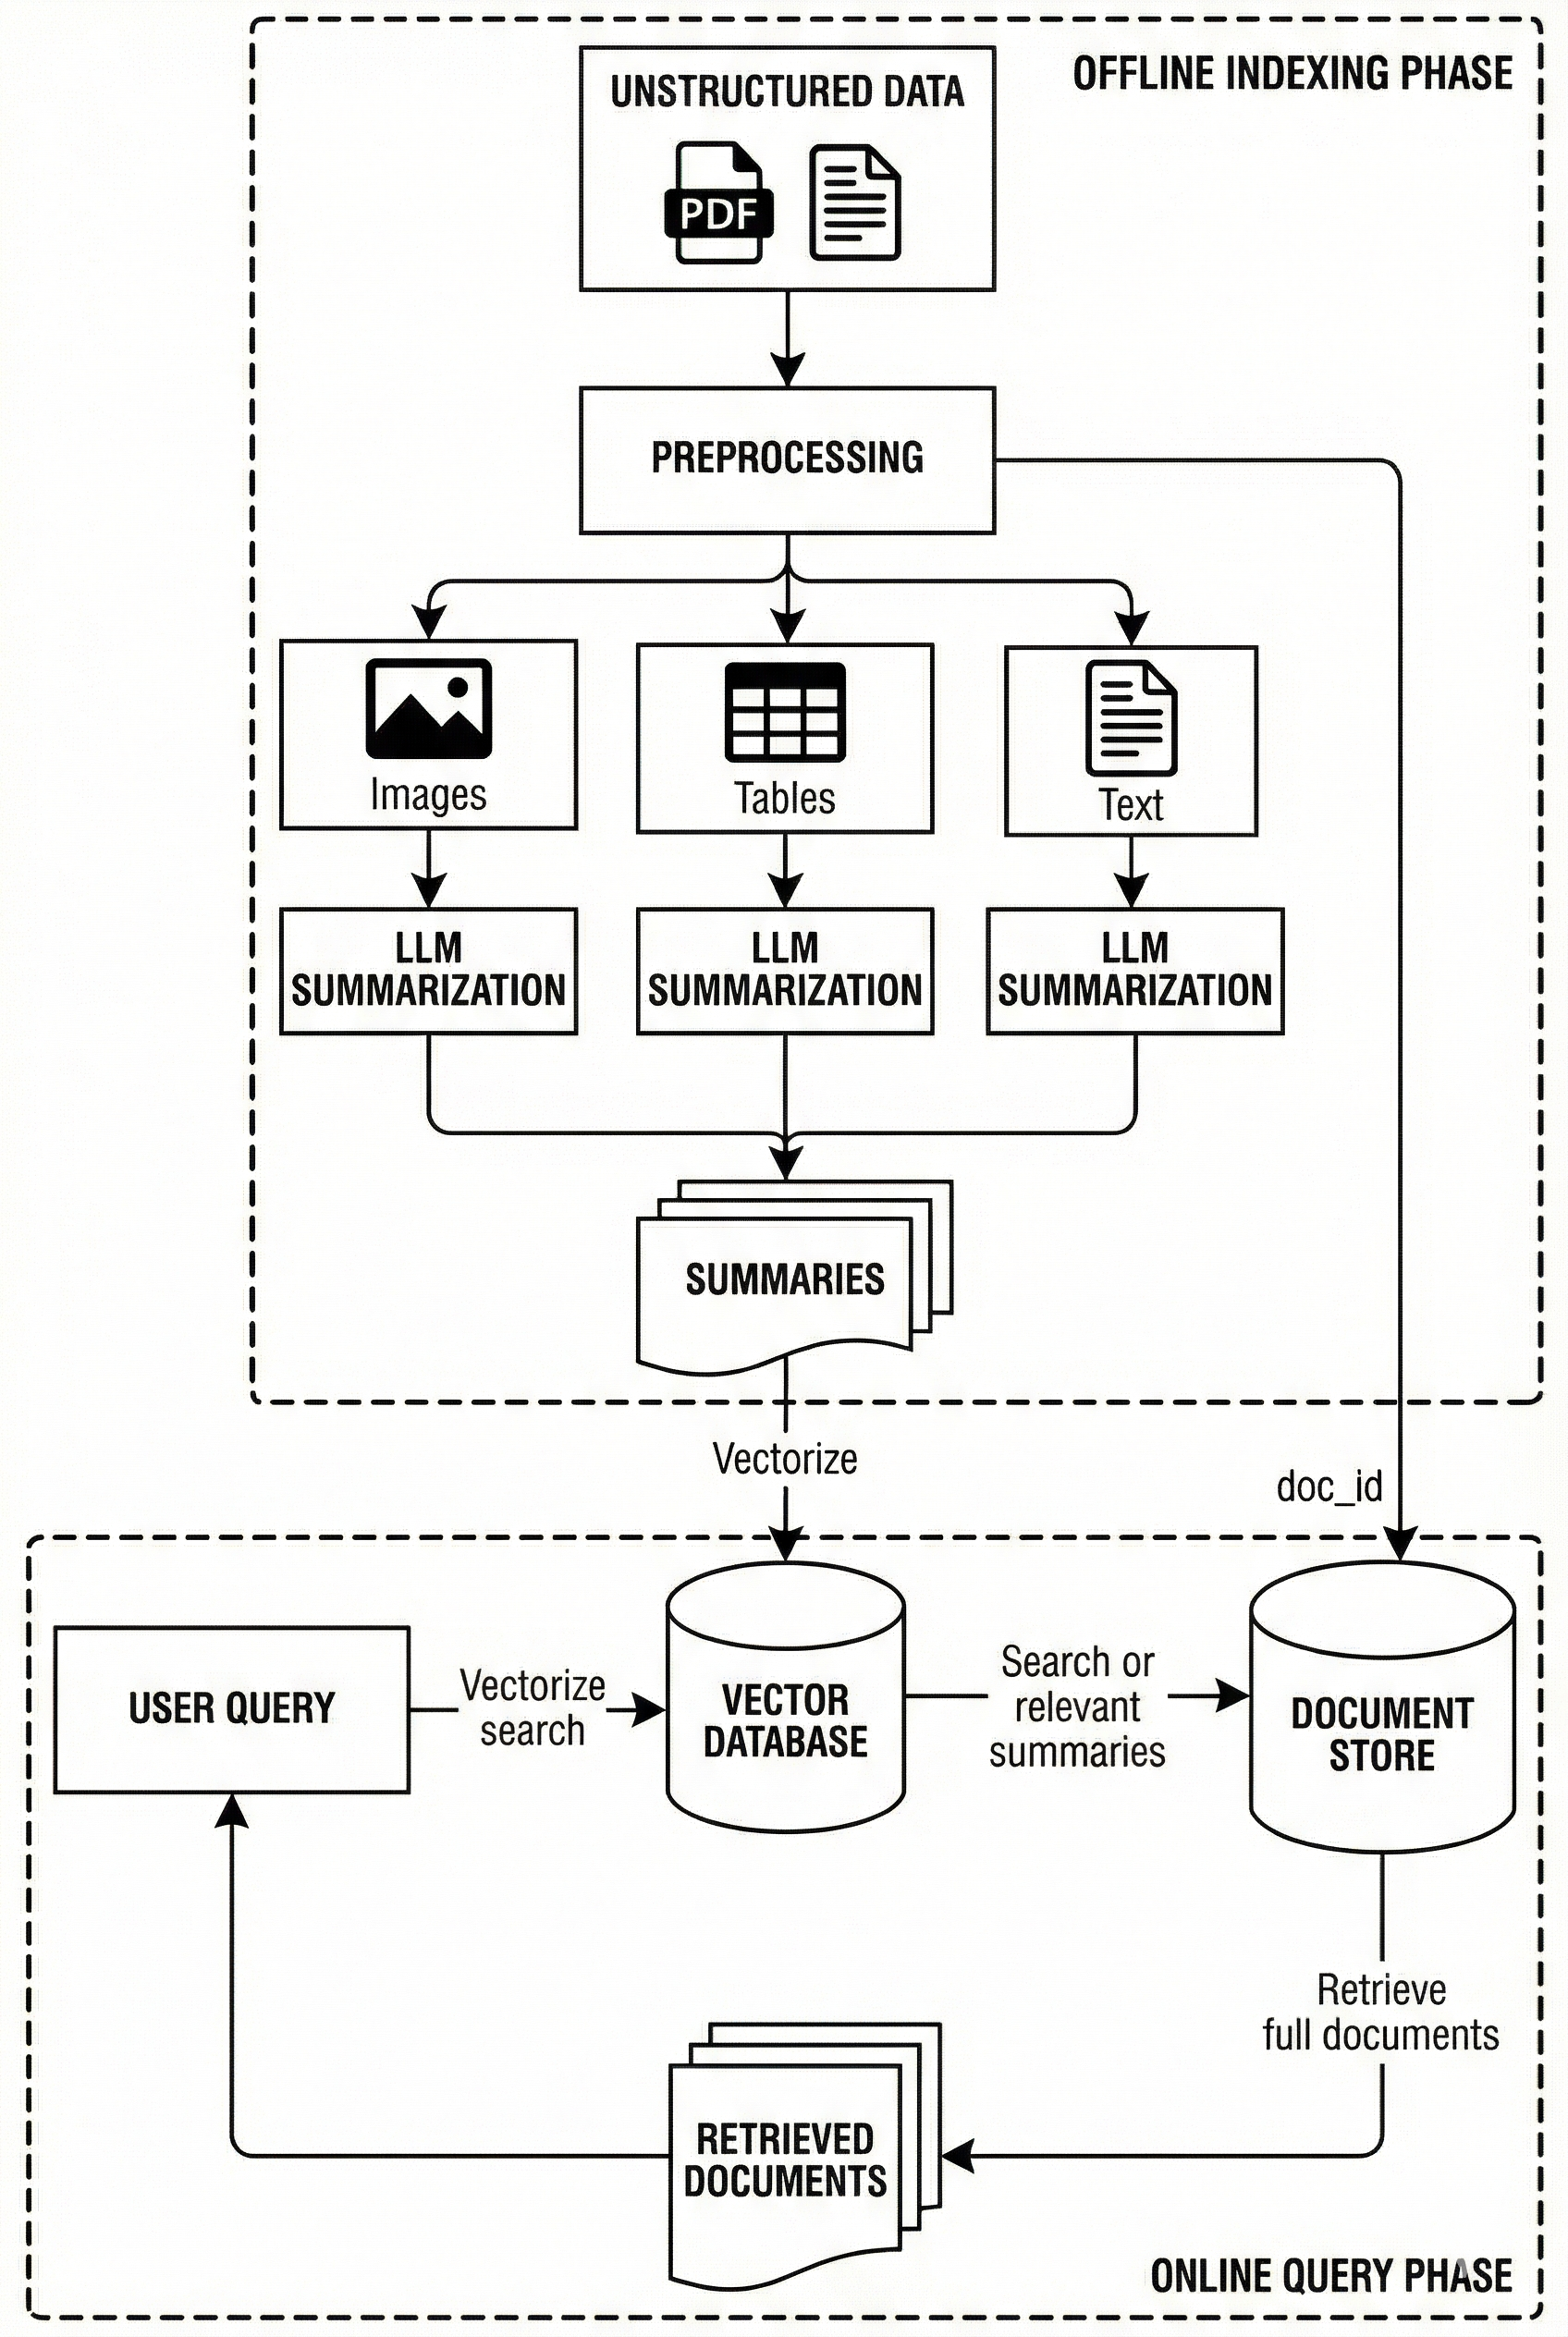
\includegraphics[width=\textwidth]{figures/rag_pipeline_diagram.png}
    \caption{Kiến trúc Advanced RAG Pipeline}
    \label{fig:rag_pipeline_diagram}
\end{figure}

Pipeline được tổ chức thành hai pha: \textbf{Indexing Phase} (offline, chạy một lần khi có tài liệu mới) và \textbf{Query Phase} (online, mỗi khi có câu hỏi từ người dùng).

\subsection{Indexing Phase: Tái cấu trúc Tri thức}

\subsubsection{Bảo toàn Cấu trúc với UnstructuredIO và Table Transformer}

Để giải quyết vấn đề  mất cấu trúc bảng biểu khi parsing, chúng tôi sử  dụng UnstructuredIO --- một thư viện mạnh mẽ cho Document Layout Analysis. Thay vì PyPDF chỉ trích xuất raw text, UnstructuredIO sử dụng computer vision để detect các regions trong PDF: Text blocks, Table regions, và Image regions. Đặc biệt, với tables, UnstructuredIO bảo toàn cấu trúc 2D bằng cách chuyển đổi thành HTML.

Cấu hình UnstructedIO được đề cập trong Annexe. 
\begin{verbatim}
# Cấu hình UnstructuredIO cho hi-res parsing
chunks = partition_pdf(
    filename=file_path,
    strategy="hi_res",              # Document Layout Analysis
    infer_table_structure=True,     # Detect và parse bảng
    extract_image_block_types=["Image", "Table"],
    chunking_strategy="by_title",   # Chunk theo section
    max_characters=10000
)
\end{verbatim}
Chúng tôi sử dụng strategy "hi\_res" của UnstructedIO. Với strategy này, UnstructuredIO coi mỗi trang tài liệu là một hình ảnh và đưa qua các mô hình Object Detection như YoloX hoặc Detectron2 để phân loại các vùng trong trang thành Title, Text, List, Table, Image và dự đoán các "bounding boxes" (khung bao) quanh từng thành phần. Đặc biệt, đối với các vùng đánh dấu là "Table", UnstructuredIO không chỉ trích xuất chữ mà còn phải hiểu cấu trúc hàng/cột nhờ vào Table Transformer (TATR). Cách hoạt động: 1. Table Detection: Xác định vị trí bảng. 2. Table Structure Recognition: Nhận diện các đường kẻ (cells), các ô bị gộp (merged cells) và phân loại đâu là Header, đâu là Body. 3. HTML Mapping: Cuối cùng, nó ánh xạ các tọa độ này thành thẻ <table> để LLM dễ dàng xử lý.

% ảnh của 1 bảng trong trang tài liệu được phát hiện và render
\begin{figure}[H]
    \centering
    \includegraphics[width=0.8\textwidth]{figures/unstructuredio_table_detection.png}
    \caption{Phát hiện và render bảng tài chính}
    \label{fig:unstructuredio_table_detection}
\end{figure}

% Ảnh một trạng tài liệu được

Kết quả: Bảng tài chính được bảo toàn dưới dạng HTML:
\begin{htmlcode}
<table>
    <thead>
        <tr>
            <th>Sous modules (en k€)</th>
            <th>SCR 2024</th>
            <th>SCR 2023</th>
            <th>Evolution</th>
        </tr>
    </thead>
    <tbody>
        <tr>
            <td>Type 1</td>
            <td>2 692</td>
            <td>2 487</td>
            <td>8%</td>
        </tr>
        <tr>
            <td>Type 2</td>
            <td>28 377</td>
            <td>36 221</td>
            <td>-22%</td>
        </tr>
        <tr>
            <td>Effet de diversification</td>
            <td>-621</td>
            <td>-586</td>
            <td>6%</td>
        </tr>
        <tr>
            <td>Risque de défaut</td>
            <td>30 448</td>
            <td>38 121</td>
            <td>-20%</td>
        </tr>
    </tbody>
</table>
\end{htmlcode}

Cũng cùng là bảng trong phần test PyPDF ở trên, nhưng bây giờ chúng ta đã giữ được cấu trúc bảng dưới dạng HTML. Cấu trúc này sẽ được feed cho LLM. Việc sử dụng HTML làm định dạng trung gian cho bảng biểu là tối ưu nhất vì các LLM hiện đại (như Gemma-3) được huấn luyện trên lượng lớn dữ liệu web, giúp chúng có khả năng "hiểu" và "suy luận" trên cấu trúc thẻ <table> tốt hơn nhiều so với văn bản thuần túy.

\subsubsection{Semantic Bridge: Cơ chế Summarization cho Dữ liệu Đa phương thức}

Để thu hẹp khoảng cách ngữ nghĩa giữa câu hỏi của người dùng và các con số khô khan trong bảng biểu/hình ảnh, chúng tôi triển khai lớp Summarization. Các embedding model hiện nay thường gặp khó khăn với:

Bảng số liệu (Tables): Các bảng quá lớn hoặc chứa số liệu thuần túy (ví dụ: "2024: 210,294") thường thiếu từ khóa ngữ cảnh (như "doanh thu", "tăng trưởng"), khiến việc truy xuất không chính xác.

Hình ảnh (Images): Embedding model truyền thống không thể "đọc" trực tiếp nội dung từ ảnh.

\textbf{Giải pháp}: Sử dụng LLM để tạo tóm tắt (Summary) cho từng chunk dữ liệu, đóng vai trò "cầu nối ngữ nghĩa" giúp tăng hiệu quả định danh nội dung.

Chúng tôi sử dụng Gemma-3-12b-it, để phân tích các bảng số liệu phức tạp trong chunk. LLM sẽ diễn giải các con số thành văn bản có ý nghĩa (ví dụ: "Bảng thể hiện doanh thu năm 2024 đạt 210.294 k€, tăng 6\%"). Điều này giúp embedding của chunk khớp chính xác với các truy vấn mang tính mô tả của người dùng. Đối với các chunk chứa hình ảnh, vì Gemma-3-12b-it là một Multimodal LM có khả năng chuyển đổi thông tin thị giác thành mô tả văn bản. Quá trình này giúp embedding model "hiểu" được nội dung ảnh thông qua lớp summary bổ trợ.

Kết quả: Summary giúp làm giàu (enrich) thông tin cho chunk, đảm bảo độ tương đồng (similarity) cao nhất giữa vector truy vấn và nội dung tài liệu, ngay cả khi dữ liệu gốc không chứa các từ khóa xuất hiện trong câu hỏi.

Đối với bảng trong hình \ref{fig:unstructuredio_table_detection}, summary được tạo ra như sau:
\begin{center}
    \fbox{
    \begin{minipage}{0.95\textwidth}
        \footnotesize
        \textbf{Summary:} "Le tableau détaille l'évolution du Solvency Capital Requirement (SCR) pour différents sous-modules entre 2023 et 2024, avec les montants exprimés en milliers d'euros (k€) et l'évolution en pourcentage. 

        Pour le sous-module << Type 1 >>, le SCR est passé de 2 487 k€ en 2023 à 2 692 k€ en 2024, affichant une évolution de 8\%. Le sous-module << Type 2 >> a vu son SCR passer de 36 221 k€ en 2023 à 28 377 k€ en 2024, avec une évolution indiquée de -22\%. 

        L'<< Effet de diversification >> a évolué de -586 k€ en 2023 à 621 k€ en 2024, soit une évolution de 6\%. Enfin, le << Risque de défaut >> a diminué, passant de 38 121 k€ en 2023 à 30 448 k€ en 2024, l'évolution diminue de -20\%."
    \end{minipage}
    }
\end{center}

Summary này trở thành ``semantic bridge'': khi người dùng hỏi về ``doanh thu 2024'', embedding của câu hỏi sẽ có similarity cao với summary (chứa ``chiffre d'affaires'' và ``2024'').

\subsubsection{Parent-Child Indexing Strategy}

\textbf{Vấn đề giải quyết}: Trade-off giữa retrieval precision và LLM context.

\textbf{Giải pháp}: Lưu summary vào VectorStore, raw content vào DocStore.

Sau bước summary generation, mỗi chunk giờ có hai phần: raw content và summary của chính nó. Summary sẽ được lưu vào vector store để  retrieval. Tuy nhiên nếu ta sử dụng chính summary này làm context cho LLM, LLM sẽ bị thiếu thông tin cần thiết để  trả lời chi tiết. Summary ngắn gọn giúp retrieval chính xác hơn (ít noise), nhưng LLM cần raw content đầy đủ (bao gồm HTML table) để sinh câu trả lời chi tiết. Vì vậy, chúng tôi áp dụng \textbf{Parent-Child Indexing Strategy}:

Quy trình:
\begin{enumerate}
    \item Index summary embeddings vào ChromaDB/Qdrant với \texttt{doc\_id} liên kết.
    \item Lưu raw content (text, HTML tables, base64 images) vào InMemoryStore.
    \item Khi retrieval, tìm summaries tương tự, sau đó fetch raw content tương ứng theo \texttt{doc\_id}.
\end{enumerate}

Bây giờ, summary sẽ chịu trách nhiệm định vị các chunk liên quan. Sau khi biết chunk nào có liên quan rồi, raw content của chunk đó sẽ được feed cho LLM để đảm bảo LLM có đủ thông tin chi tiết để trả lời câu hỏi. Strategy này có lợi thế: retrieval phase chính xác và nhanh hơn vì summary chứa đầy đủ thông tin nhưng ngắn gọn hơn raw content, đồng thời LLM có đầy đủ context từ raw content.

\subsubsection{Multilingual Embedding Model}

Trong phần trê, chúng tôi có đề cập rằng embedding model all-Mini-LM6 không thể hiện tốt trên những ngôn ngữ khác tiếng Anh vì nó được train chủ yếu trên dữ liệu tiếng Anh. Ở đây chúng tôi muốn một embedding model hiểu được nhiều thứ tiếng (cụ thể trong trường hợp của chúng tôi là các tài liệu tiếng Pháp), tuy nhiên model đó vẫn phải đáp ứng điều kiện nhỏ gọn (dưới 1B tham số). Dựa trên bảng xếp hạng MTEB, chúng tôi lựa chọn \texttt{intfloat/multilingual-e5-large-instruct}. Hình \ref{fig:mteb_multilingual} so sánh hiệu suất của các model phổ biến trên tập dữ liệu multilingual MTEB:

\begin{figure}[H]
    \centering
    \includegraphics[width=0.8\textwidth]{figures/mteb_multilingual_comparison.png}
    \caption{So sánh hiệu suất các embedding model trên MTEB Multilingual}
    \label{fig:mteb_multilingual}
\end{figure}

Model này có 560M parameters, được train trên 100+ ngôn ngữ với instruction-following capability. Ở thời điểm xây dựng pipeline, đây là model retriever tốt nhất dưới 1B parameters cho dữ liệu đa ngôn ngữ (Lưu ý: hiện tại đã có các model mới ra đời như \texttt{Qwen3-embeddings-0.6B} có thể  sử dụng thay thế để tối ưu pipeline).

% Đặc biệt, nó cho phép prefix query với task description:

% \begin{verbatim}
% query = get_detailed_instruct(
%     "Given a query, retrieve relevant passages that answer the query.",
%     "Quel est le chiffre d'affaires 2024?"
% )
% \end{verbatim}

% Instruction này giúp model hiểu mục tiêu không chỉ là tìm passages tương tự mà là tìm passages chứa \textbf{câu trả lời}.

\subsection{Query Phase: Cơ chế Truy vấn và Tổng hợp Tri thức Đa phương thức}
Nếu Indexing Phase là quá trình xây dựng "thư viện" tri thức, thì Query Phase quyết định khả năng "tìm kiếm và diễn giải" thông tin để đưa ra câu trả lời chính xác. Để khắc phục triệt để các hạn chế của Simple RAG, chúng tôi triển khai một quy trình truy vấn hai giai đoạn (Two-stage Retrieval) kết hợp với khả năng suy luận đa phương thức.
\subsubsection{Hybrid Search: Kết hợp Semantic và Keyword}

Như đã phân tích tại phần 2.3, các truy vấn chứa mã định danh (như mã CCAM "HAFA008") thường thất bại trong không gian Vector (Dense Search) do tính chất phân tán của embedding. Để giải quyết vấn đề này, chúng tôi áp dụng chiến lược Hybrid Search, kết hợp sức mạnh của truy vấn ngữ nghĩa và truy vấn từ khóa (Sparse Search).

Cơ chế phối hợp: Chúng tôi sử dụng thuật toán BM25 để bắt chính xác các từ khóa đặc hiệu (exact match) và Dense Search với model multilingual-e5-large để hiểu ngữ cảnh.

Hợp nhất kết quả bằng Reciprocal Rank Fusion (RRF): Do thang điểm của BM25 và Vector Similarity không đồng nhất, chúng tôi sử dụng kỹ thuật RRF để xếp hạng lại các tài liệu từ cả hai nguồn. Công thức RRF giúp ưu tiên các tài liệu xuất hiện ở vị trí cao trong cả hai danh sách mà không cần chuẩn hóa điểm số:

\[
\text{RRF}(d) = \sum_{r \in R} \frac{1}{k + r(d)}
\]

Trong đó $r(d)$ là thứ hạng của tài liệu $d$, và $k$ là hằng số (thường chọn $k=60$) để giảm nhiễu từ các tài liệu có thứ hạng cực thấp. 

Chúng tôi sử dụng Qdrant với Hybrid Search:

\begin{verbatim}
vector_store = QdrantVectorStore(
    client=client,
    collection_name="general_usecase",
    enable_hybrid=True,
    fastembed_sparse_model="Qdrant/bm25"
)
\end{verbatim}

\subsubsection{Cross-Encoder Reranking: Giải quyết hiện tượng "Lost in the Middle"}

Mặc dù Hybrid Search cải thiện đáng kể khả năng thu hồi (Recall), nhưng danh sách kết quả vẫn có thể chứa nhiễu. LLM khi đối mặt với quá nhiều thông tin trong context window thường gặp hiện tượng suy giảm hiệu suất ở các vị trí giữa (Lost in the Middle). Nếu chunk chứa thông tin rơi vào các vị trí giữa này, LLM sẽ có xu hướng bỏ qua và tìm kiếm ở những chunk vị trí đầu hoặc cuối trong context. Chúng tôi giải quyết vấn đề này bằng một lớp Reranker sử dụng kiến trúc Cross-Encoder.

Sự khác biệt về kiến trúc: Khác với Bi-Encoder (dùng trong Indexing) chỉ tính toán similarity dựa trên hai vector độc lập, Cross-Encoder đưa đồng thời cả Query và Document vào mô hình Transformer. Điều này cho phép mô hình thực hiện cơ chế Full Self-Attention giữa mọi token của câu hỏi và tài liệu, từ đó đánh giá mức độ liên quan một cách cực kỳ chi tiết.

Chiến lược tối ưu: Do chi phí tính toán của Cross-Encoder lớn, chúng tôi chỉ thực hiện tái xếp hạng trên top-10 ứng viên từ bước Hybrid Search. Kết quả là những passage có độ tương quan cao nhất sẽ được đưa lên đầu ngữ cảnh, tối ưu hóa khả năng "đọc hiểu" của LLM ở bước sau.

% Ở phần trên, chúng tôi đã đề cập đến vấn đề Lost in the Middle --- LLM bỏ qua thông tin giữa context. Giải pháp cho vấn đề này chính là sử dụng model Reranker để đưa thông tin relevant nhất lên đầu. Reranker sử dụng model có kiến trúc cross encoder, cho phép đưa cặp (query, document) vào cùng một Transformer, cho phép attention giữa mọi token --- đánh giá relevance chính xác hơn so với bi-encoder (được sử dụng trong Dense Search). Sở dĩ chúng tôi không dùng cross-encoder trực tiếp trong retrieval phase vì chi phí tính toán quá cao (phải encode từng cặp query-document cho tất cả các chunk). Chúng tôi chỉ dùng cross-encoder để rerank top-10 candidates sau retrieval phase. Lúc này chỉ cần encode 10 cặp, chi phí chấp nhận được.

% Quy trình này diễn ra như sau: 
% \begin{enumerate}
%     \item Hybrid Search retrieve top-10 candidates (nhanh vì dùng HNSW index).
%     \item Cross-Encoder (\texttt{cross-encoder/ms-marco-MiniLM-L-12-v2}) score 10 candidates này.
%     \item Chọn top-5 có score cao nhất để đưa vào LLM.
% \end{enumerate}

% Với top-5 reranked results, thông tin quan trọng nhất được đảm bảo đẩy lên đầu context --- giảm thiểu ``Lost in the Middle''.

\subsubsection{Multimodal Generation: Tổng hợp tri thức từ Văn bản, Bảng biểu và Hình ảnh}

Giai đoạn cuối cùng là quá trình sinh phản hồi, nơi LLM phải đóng vai trò một chuyên gia tổng hợp dữ liệu đa nguồn. Thay vì chỉ nhận văn bản thuần túy (plain text) như Simple RAG, mô hình Gemma-3-12b-it của chúng tôi được cung cấp một "Augmented Prompt" giàu cấu trúc:

Cấu trúc 2D: Các bảng biểu tài chính được truyền dưới dạng HTML nguyên bản, giúp LLM duy trì sự gióng hàng giữa các cột (năm tài chính) và hàng (chỉ số doanh thu), loại bỏ hoàn toàn lỗi đọc sai số liệu do làm phẳng văn bản (flattening).

Thông tin thị giác: Đối với các chunk chứa biểu đồ hoặc hình ảnh minh họa y tế, mô hình nhận trực tiếp dữ liệu hình ảnh (Base64) cùng với các đoạn mô tả (summaries) đã tạo ở bước Indexing.

Hàng rào an toàn (Guardrails): Prompt được thiết kế theo kỹ thuật Chain-of-Thought (CoT), yêu cầu mô hình trích dẫn trực tiếp nguồn dữ liệu từ ngữ cảnh để giảm thiểu hiện tượng ảo giác (hallucination).

Kết quả là pipeline này không chỉ trả về câu trả lời mà còn giải thích được "tại sao số liệu đó được chọn" dựa trên việc đối chiếu giữa bảng biểu và văn bản mô tả xung quanh. Điều này tạo ra sự minh bạch — một yếu tố then chốt trong các quyết định tài chính và chẩn đoán y khoa.

\section{Đánh giá Thực nghiệm}

Để chứng minh tính hiệu quả của kiến trúc Advanced RAG đề xuất, chúng tôi tiến hành đánh giá định lượng trên hai bộ dữ liệu thực tế từ đối tác, đồng thời thực hiện nghiên cứu bóc tách (Ablation Study) để xác định giá trị đóng góp của từng thành phần kỹ thuật.

\subsection{Thiết lập Thực nghiệm}

\subsubsection{Tập dữ liệu Kiểm thử (Testbeds)}

GPM Test Set: Bao gồm 25 cặp câu hỏi - câu trả lời (Q\&A) được gán nhãn thủ công bởi các chuyên gia tài chính từ tài liệu AGMF. Tập dữ liệu này tập trung vào khả năng truy xuất số liệu và suy luận trên bảng biểu.

CCAM Test Set: Bao gồm 10 kịch bản tư vấn lâm sàng (Consultation Scenarios) phức tạp. Mỗi kịch bản yêu cầu hệ thống đề xuất đúng mã CCAM mục tiêu, được xác thực bởi chính bác sĩ Besnier.

\subsubsection{Hệ thống Chỉ số Đánh giá (Metrics)}

Chúng tôi sử dụng khung đánh giá RAGAS (RAG Assessment) kết hợp với phương pháp LLM-as-a-Judge để đảm bảo tính khách quan:
Faithfulness (Tính trung thực): Đo lường mức độ câu trả lời được dẫn chứng trực tiếp từ ngữ cảnh (context), nhằm kiểm soát hiện tượng ảo giác.
Answer Relevancy (Sự phù hợp): Đánh giá mức độ trực diện và đầy đủ của câu trả lời đối với truy vấn của người dùng.
Answer Correctness (Độ chính xác nội dung): So sánh ngữ nghĩa giữa câu trả lời của hệ thống và Ground-truth (thang điểm 0-1).
Context Precision: Đánh giá khả năng của Retriever trong việc đưa các chunk thông tin hữu ích lên vị trí đầu danh sách.
Code Hit Rate@k (Dành cho CCAM): Tỷ lệ mã CCAM chính xác xuất hiện trong top $k$ kết quả truy xuất.

\subsection{Kết quả So sánh: Simple RAG vs. Advanced RAG}

Kết quả thực nghiệm trên tập dữ liệu GPM cho thấy sự vượt trội toàn diện của kiến trúc nâng cao:

\begin{table}[H]
    \centering
    \caption{Kết quả trên GPM Test Set (25 câu hỏi)}
    \begin{tabular}{|l|c|c|c|c|}
        \hline
        \textbf{Pipeline} & \textbf{Precision} & \textbf{Relevancy} & \textbf{Faithfulness} & \textbf{Context Precision} 
         \\
        \hline
        Simple RAG & 0.648 & 0.788 & 0.732 & 0.654
         \\
        \hline
        Advanced RAG & \textbf{0.82} & \textbf{0.88} & \textbf{0.84} & \textbf{0.76} \\
        \hline
        \textit{Improvement} & \textit{+26.54\%} & \textit{+11.68\%} & \textit{+14.22\%} & \textit{+16.83\%} \\
        \hline
    \end{tabular}
\end{table}

Sự gia tăng mạnh mẽ nhất nằm ở Context Precision (+35.3\%) và Answer Correctness (+34.1\%). Điều này chứng minh rằng việc bảo toàn cấu trúc bảng biểu qua UnstructuredIO và cơ chế Reranking đã giúp LLM tiếp cận đúng và đủ thông tin cần thiết, thay vì phải "đoán" dựa trên các mảnh vụn văn bản như ở bản Baseline.

Đối với bài toán CCAM, kết quả cũng ghi nhận sự thay đổi mang tính bước ngoặt nhờ cơ chế Hybrid Search:

\begin{table}[H]
    \centering
    \caption{Kết quả trên CCAM Test Set (10 scenarios)}
    \begin{tabular}{|l|c|c|}
        \hline
        \textbf{Pipeline} & \textbf{Code Hit Rate@5} & \textbf{Code Hit Rate@20} \\
        \hline
        Simple RAG (Dense only) & 0.42 & 0.65 \\
        \hline
        Advanced RAG (Hybrid + Rerank) & \textbf{0.78} & \textbf{0.92} \\
        \hline
        \textit{Improvement} & \textit{+85.7\%} & \textit{+41.5\%} \\
        \hline
    \end{tabular}
\end{table}

Code Hit Rate@k đo tỷ lệ ground-truth code xuất hiện trong top-k retrieved passages. Hybrid Search với BM25 mang lại cải thiện đáng kể nhờ exact matching với mã CCAM.

\section{Ablation Study: Đóng góp của Từng Thành phần}

Để hiểu rõ contribution của từng thành phần, chúng tôi thực hiện ablation study: bắt đầu từ Simple RAG baseline, lần lượt thêm từng component và đo sự cải thiện.

\begin{table}[H]
    \centering
    \caption{Ablation Study trên GPM Test Set}
    \begin{tabular}{|l|c|c|c|}
        \hline
        \textbf{Configuration} & \textbf{Precision} & \textbf{$\Delta$ vs Baseline} & \textbf{Cumulative $\Delta$} \\
        \hline
        Baseline (Simple RAG) & 0.728 & --- & --- \\
        \hline
        + UnstructuredIO Parsing & 0.792 & +8.8\% & +8.8\% \\
        \hline
        + Summarization & 0.836 & +5.6\% & +14.8\% \\
        \hline
        + Multilingual E5 Embedding & 0.884 & +5.7\% & +21.4\% \\
        \hline
        + Hybrid Search & 0.924 & +4.5\% & +26.9\% \\
        \hline
        + Reranking & \textbf{0.976} & +5.6\% & \textbf{+34.1\%} \\
        \hline
    \end{tabular}
\end{table}

\subsection{Phân tích Chi tiết từng Component}

\textbf{UnstructuredIO Parsing (+8.8\%)}: Đây là thành phần đóng góp quan trọng nhất. Việc chuyển đổi bảng tài chính sang HTML giúp LLM thực hiện phép ánh xạ (mapping) chính xác giữa các tiêu đề cột và giá trị dòng.

\textbf{Summarization \& E5 (+11.3\% combined)}: Việc kết hợp giữa tóm tắt nội dung (làm giàu ngữ nghĩa) và mô hình Embedding đa ngôn ngữ giúp hệ thống vượt qua rào cản về ngôn ngữ (tiếng Pháp) và sự khan hiếm từ khóa trong các bảng số liệu.

\textbf{Hybrid Search \& Reranking (+10.1\% combined)}: Hai thành phần này đóng vai trò "màng lọc tinh". Hybrid Search giải quyết các truy vấn chứa mã code, trong khi Reranking đảm bảo các thông tin quan trọng không bị trôi vào giữa ngữ cảnh (tránh lỗi Lost in the Middle).


\section{Thảo luận và Hạn chế}

\subsection{Ưu điểm và Đóng góp}

Hệ thống đã chứng minh được tính khả thi trong việc xây dựng một Pipeline RAG thống nhất cho đa miền (Tài chính \& Y tế). Việc triển khai hoàn toàn Local không chỉ đáp ứng tiêu chuẩn bảo mật dữ liệu nghiêm ngặt mà còn tối ưu hóa chi phí vận hành lâu dài cho doanh nghiệp.

\subsection{Hạn chế tồn tại}

Độ trễ (Latency): Việc sử dụng Cross-Encoder làm tăng đáng kể thời gian xử lý (tăng khoảng 1.5s - 3s cho mỗi truy vấn). Ngoài ra việc sử dụng Multimodal LM để tóm tắt cũng làm tăng thời gian processing dữ liệu đầu vào. Đây là một trade-off giữa độ chính xác và tốc độ.

Kích thước mẫu thử: Tập test 25 và 10 scenarios là tương đối nhỏ để đánh giá khả năng tổng quát hóa (generalization) trên toàn bộ mọi loại biểu mẫu tài chính/y tế hiện có.

\subsection{Hướng Phát triển}

\begin{itemize}
    \item \textbf{Adaptive Hybrid Search}: Classifier tự động điều chỉnh trọng số Dense/Sparse dựa trên query type.
    \item \textbf{Query Routing}: Route semantic queries đến Dense-heavy path, code queries đến Sparse-heavy path.
    \item \textbf{Caching và Optimization}: Cache summaries và embeddings để giảm latency.
\end{itemize}

\section{Kết luận Chương}

Chương này đã trình bày chi tiết quá trình phát triển kiến trúc Advanced RAG nhằm giải quyết bài toán hiểu tài liệu phức tạp trong môi trường doanh nghiệp. Thông qua việc phân tích thực nghiệm các điểm yếu của Simple RAG, chúng tôi đã đề xuất một quy trình cải tiến tập trung vào ba trụ cột: Bảo toàn cấu trúc (Parsing), Làm giàu ngữ nghĩa (Summarization) và Truy xuất đa tầng (Hybrid Search \& Reranking).

Kết quả thực nghiệm khẳng định tính đúng đắn của phương pháp với mức cải thiện 34.1\% về độ chính xác câu trả lời và 85.7\% khả năng tìm kiếm mã định danh chuyên ngành. Những đóng góp này không chỉ giải quyết yêu cầu cấp bách của đối tác Torus AI mà còn đóng góp một framework thực tiễn cho cộng đồng nghiên cứu RAG trên dữ liệu đa phương thức.

%%------------------------------- chapter ------------------------------------


\chapter{Fine-tuning Mô hình Ngôn ngữ Nhỏ cho Tác vụ Đặc thù: Trường hợp Tarot Reader}

Chương 3 đã trình bày giải pháp Advanced RAG nhằm thu hẹp Khoảng cách Tri thức (Knowledge Gap), đảm bảo hệ thống AI có thể truy xuất chính xác các thông tin chuyên biệt từ dữ liệu doanh nghiệp. Tuy nhiên, trong thực tế triển khai các ứng dụng AI hướng tới người dùng cuối (User-centric AI), chúng tôi nhận thấy rằng tính chính xác của thông tin chỉ là điều kiện cần. Để một hệ thống AI thực sự được chấp nhận, nó cần giải quyết một thách thức khó khăn hơn: Khoảng cách Hành vi (Behavior Gap).

Khoảng cách này bộc lộ rõ nét khi chúng tôi thực hiện dự án xây dựng Tarot Reader — một hệ thống hỗ trợ tư vấn tâm lý và giải trí dựa trên bộ bài Tarot. Tại đây, vấn đề không còn là trích xuất dữ liệu từ một bảng biểu tài chính, mà là làm thế nào để mô hình duy trì một phong cách giao tiếp nhất quán, tuân thủ nghiêm ngặt quy trình tư vấn (ritualistic workflow) và thể hiện được sự thấu cảm (empathy) phù hợp với vai trò của một chuyên gia tâm lý hoặc một người đọc bài Tarot chuyên nghiệp.

Trong dự án này, chúng tôi đối mặt với một thực tế: Các mô hình ngôn ngữ lớn (LLM) như GPT-4, dù rất thông minh, thường có xu hướng trả lời quá chi tiết, máy móc hoặc dễ dàng "thoát vai" (out-of-character) khi cuộc hội thoại kéo dài. Hơn nữa, chi phí vận hành các mô hình lớn cho một ứng dụng mang tính giải trí cá nhân là không tối ưu.

Vì vậy, Chương 4 sẽ tập trung vào kỹ thuật Fine-tuning các Mô hình Ngôn ngữ Nhỏ (SLMs - Small Language Models). Chúng tôi đặt mục tiêu chứng minh rằng: Một mô hình với kích thước chỉ từ 0.5B đến 1.5B tham số, nếu được huấn luyện đúng cách, có thể đạt được sự nhất quán về hành vi và phong cách vượt trội so với các mô hình lớn chỉ sử dụng Prompt Engineering, đồng thời đáp ứng các tiêu chuẩn khắt khe về độ trễ và chi phí triển khai.

\section{Phân tích Bài toán: Tại sao Prompt Engineering là chưa đủ?}

\subsection{Giới hạn của In-Context Learning đối với Tác vụ Hành vi}

Một hướng tiếp cận tự nhiên cho chatbot Tarot là sử dụng các mô hình mạnh như GPT-4o hay Claude 3.5 với system prompt được thiết kế cẩn thận. Tuy nhiên, qua thử nghiệm thực tế, chúng tôi nhận thấy ba rào cản kỹ thuật:

\textbf{Attention Dilution} Mặc dù các mô hình hiện đại hỗ trợ context window lớn (như 128K tokens của GPT-4), nghiên cứu thực nghiệm về hiện tượng \textit{``Lost in the Middle''} (Liu et al., 2023) chỉ ra rằng hiệu suất của mô hình giảm đáng kể khi các thông tin hướng dẫn quan trọng bị chìm trong một context quá dài. Một cuộc hội thoại Tarot điển hình kéo dài 1500--2000 tokens; để bao quát đủ các sắc thái---từ giọng điệu, cách đặt câu hỏi mở, đến xử lý người dùng hoài nghi---chúng ta cần hàng chục ví dụ (few-shot), ý nghĩa các lá bài cũng như định hình phong cách ngôn ngữ, kỹ thuật đặt câu hỏi cũng như quy trình. Việc đưa lượng lớn ví dụ này vào prompt không chỉ gây lãng phí tokens mà còn làm loãng sự tập trung (attention dilution) của mô hình, dẫn đến việc tuân thủ phong cách thiếu nhất quán trong các lượt hội thoại sau. Ngoài ra, việc model chỉ làm theo một cách máy móc và rập khuôn theo các ví dụ mà không có sự sáng tạo cũng là một vấn đề của in context learning.

\textbf{Hạn chế về chi phí vận hành.} Bảng \ref{tab:cost-comparison} so sánh chi phí giữa các phương án. Với một ứng dụng xử lý 10.000 cuộc hội thoại/tháng (quy mô nhỏ-vừa), chi phí API của GPT-4 dao động \$300--900/tháng. Mô hình fine-tuned chạy trên GPU cloud chỉ tốn 10--20\% con số đó, đồng thời cho phép kiểm soát hoàn toàn về dữ liệu và hành vi.

\begin{table}[H]
    \centering
    \begin{tabular}{|l|c|c|}
        \hline
        \textbf{Phương án} & \textbf{Chi phí/1K tokens} & \textbf{Chi phí/tháng*} \\
        \hline
        GPT-4-turbo API & \$0.01--0.03 & \$300--900 \\
        Claude 3 Sonnet API & \$0.003--0.015 & \$90--450 \\
        Qwen-1.5B Fine-tuned (T4) & \$0.0005** & \$50--100 \\
        Qwen-0.5B Fine-tuned (Edge) & \$0.0001** & \$10--30  \\
        \hline
    \end{tabular}
    \caption{So sánh chi phí vận hành. *Giả định 10K cuộc hội thoại × 3K tokens/cuộc. **Chi phí GPU amortized.}
    \label{tab:cost-comparison}
\end{table}

% Để tối ưu chi phí GPU, chúng tôi sử dụng engine suy luận vLLM với kỹ thuật PagedAttention, cho phép đạt throughput trên 100 tokens/s ngay cả với GPU dòng cũ như NVIDIA T4

\textbf{Hạn chế về độ trễ.} API cloud thường có latency 500ms--2s cho token đầu tiên, tạo cảm giác ``chờ đợi'' không phù hợp với trải nghiệm real-time của ứng dụng tư vấn. Mô hình nhỏ chạy local có thể đạt time-to-first-token dưới 100ms, mang lại cảm giác phản hồi tức thì.

\subsection{Đặc thù của Tác vụ Tarot Reader}

Tarot Reader không phải là một chatbot thông tin, mà là một thực thể có "Character". Tác vụ này đòi hỏi sự tích hợp chặt chẽ giữa ba lớp thông tin:

Lớp Tri thức (Knowledge Layer): Ý nghĩa của 78 lá bài trong cả hai trạng thái xuôi và ngược.

Lớp Quy trình (Operational Layer): Tuân thủ workflow nghiêm ngặt: Chào hỏi → Khám phá vấn đề → Mời rút bài → Diễn giải từng lá → Tổng hợp thông điệp.

Lớp Cảm xúc (Emotional Layer): Sử dụng ngôn ngữ thấu cảm, đặt câu hỏi gợi mở thay vì khẳng định cứng nhắc.

\subsection{Câu hỏi Nghiên cứu}

Từ phân tích trên, chúng tôi quyết định sử dụng Data-centric Fine-tuning để "đúc" (bake) toàn bộ các lớp hành vi này vào trọng số của mô hình nhỏ, biến nó thành một chuyên gia thực thụ trong lĩnh vực của mình. Chúng tôi đặt ra hai câu hỏi nghiên cứu chính:

\begin{itemize}
    \item \textbf{RQ1:} Liệu mô hình nhỏ ($\leq$ 3B tham số-) được fine-tune có thể đạt behavioral consistency tương đương hoặc tốt hơn LLM lớn với prompt engineering?
        
    \item \textbf{RQ2:} LoRA có đủ để học behavioral patterns hay cần full fine-tuning?
\end{itemize}

\section{Phương pháp: Data-Centric Fine-tuning Pipeline}

Hình \ref{fig:finetuning-pipeline} minh họa pipeline của chúng tôi, gồm ba giai đoạn: (1) Tạo dữ liệu tổng hợp với Teacher Model, (2) Supervised Fine-Tuning với LoRA/Full, và (3) Đánh giá đa chiều.

\begin{figure}[H]
    \centering
    \fbox{\parbox{0.95\textwidth}{\centering
        \textbf{[PLACEHOLDER: Pipeline Diagram]}\\[3mm]
        \begin{tabular}{ccccc}
        \fbox{\parbox{2.5cm}{\centering \small Teacher Model\\(GPT-4o, Qwen-Plus)}} & 
        $\xrightarrow{\text{sinh}}$ & 
        \fbox{\parbox{2.5cm}{\centering \small Synthetic\\Conversations}} & 
        $\xrightarrow{\text{lọc}}$ & 
        \fbox{\parbox{2.5cm}{\centering \small Training\\Dataset}} \\
        & & & & $\downarrow$ \\
        \fbox{\parbox{2.5cm}{\centering \small LLM Judge +\\Human Eval}} & 
        $\xleftarrow{\text{đánh giá}}$ & 
        \fbox{\parbox{2.5cm}{\centering \small Fine-tuned\\Model}} & 
        $\xleftarrow{\text{train}}$ & 
        \fbox{\parbox{2.5cm}{\centering \small Student Model\\+ LoRA}}
        \end{tabular}
    }}
    \caption{Pipeline Fine-tuning cho Tarot Reader. Teacher Model sinh dữ liệu mẫu, Student Model học từ dữ liệu này, kết quả được đánh giá bởi LLM Judge và human evaluators.}
    \label{fig:finetuning-pipeline}
\end{figure}

\subsection{Sinh Dữ liệu Tổng hợp: Distillation ở Tầng Hành vi}

\subsubsection{Mục tiêu và Định dạng Dữ liệu}

Thách thức đầu tiên chúng tôi đối mặt là không có sẵn bộ dữ liệu hội thoại Tarot chất lượng cao. Những cuộc hội thoại thực tế giữa người đọc bài và khách hàng vừa hiếm, vừa nhạy cảm về quyền riêng tư. Giải pháp của chúng tôi là áp dụng Knowledge Distillation ở một tầng khác biệt so với cách tiếp cận truyền thống: thay vì distill logits hay hidden states, chúng tôi distill \textit{behavioral patterns} --- tức cách ứng xử, giọng điệu, và quy trình làm việc của một chuyên gia Tarot.

Cụ thể, chúng tôi sử dụng GPT-4o và Qwen-Plus làm Teacher Model để sinh các cuộc hội thoại mẫu thể hiện đầy đủ ba lớp thông tin cần thiết: tri thức về 78 lá bài, quy trình tư vấn năm bước, và phong cách giao tiếp thấu cảm. Hai teacher model này được chọn vì khả năng tuân theo instruction phức tạp và hỗ trợ đa ngôn ngữ --- yếu tố quan trọng cho việc mở rộng sang đa ngôn ngữ sau này.

Trước khi tiến hành sinh dữ liệu, chúng tôi thu thập thông tin chi tiết về 78 lá bài Tarot từ các nguồn (dẫn nguồn), bao gồm tên lá bài, phân loại (Major/Minor Arcana), ý nghĩa khi thuận và ngược, cùng mô tả hình ảnh biểu tượng. Dữ liệu này được đưa vào context của Teacher Model để đảm bảo độ chính xác trong các phần giải nghĩa bài.


Trước khi sinh dữ liệu, cần xác định rõ dữ liệu cần có dạng như thế nào. Một cuộc hội thoại Tarot điển hình có cấu trúc như sau:

\begin{tcolorbox}[breakable, colback=gray!5!white, colframe=gray!50!black, title=\textbf{Ví dụ minh họa: Hội thoại Tarot}]
    \small
    \textbf{Querent:} Hi, I've been feeling stuck in my job lately. I'm not sure if I should stay or look for something new.

    \vspace{0.5em} % Tạo khoảng cách nhỏ giữa các lượt lời
    \textbf{Chatbot:} Hey there! Career crossroads can be tricky, right? Before we dive into the cards, tell me a bit more --- what's making you feel stuck? Is it the work itself, the environment, or something else?

    \vspace{0.5em}
    \textbf{Querent:} It's mostly that I don't feel challenged anymore. The pay is good but I'm just going through the motions.

    \vspace{0.5em}
    \textbf{Chatbot:} Ah, the golden handcuffs situation! That's actually really common. So you're craving growth and meaning, not just a paycheck. Got it. Ready to see what the cards have to say? Focus on your question, take a deep breath, and pick three cards when you're ready.

    \vspace{0.5em}
    \textbf{Querent:} [Draws: The Tower (reversed), Eight of Cups, The Star]

    \vspace{0.5em}
    \textbf{Chatbot:} Ooh, interesting spread! Let's start with The Tower reversed in your first position. Usually The Tower upright is about sudden upheaval, but reversed? It's more like... you're \textit{avoiding} a necessary change. Maybe you already know things need to shake up, but you're holding on because it feels safer?
    
    The Eight of Cups in the middle --- this one's literally about walking away from something that no longer fulfills you. See how the figure is leaving those cups behind? That's you, being called to seek something more meaningful...
    
    \textit{[continues with card interpretations and synthesis]}
\end{tcolorbox}

Cấu trúc này thể hiện đầy đủ các yêu cầu: phong cách casual (``golden handcuffs'', ``Ooh, interesting spread!''), quy trình đúng (hỏi trước, mời rút bài, giải từng lá), và sự đồng cảm (``That's actually really common'').

\subsubsection{Thu thập Tri thức về Tarot Cards}

Để Teacher Model có thể sinh dữ liệu chính xác, chúng tôi thu thập thông tin chi tiết về 78 lá bài từ các nguồn uy tín. Dữ liệu được crawl bằng thư viện BeautifulSoup4 và lưu dưới dạng CSV với các trường: \texttt{card\_name}, \texttt{card\_box} (Major/Minor Arcana), \texttt{upright} (ý nghĩa khi thuận), \texttt{reversed} (ý nghĩa khi ngược), \texttt{description} (mô tả hình ảnh và biểu tượng), và \texttt{img\_url}. Chi tiết về code crawling được trình bày trong Phụ lục.

\begin{table}[H]
    \centering
    \small
    \begin{tabular}{|l|l|p{4cm}|p{4cm}|}
        \hline
        \textbf{Card} & \textbf{Type} & \textbf{Upright} & \textbf{Reversed} \\
        \hline
        The Fool & Major & Beginnings, innocence, spontaneity, free spirit & Holding back, recklessness, risk-taking \\
        The Tower & Major & Sudden change, upheaval, revelation & Fear of change, avoiding disaster \\
        Eight of Cups & Minor & Walking away, seeking truth, leaving behind & Fear of change, stagnation \\
        \hline
    \end{tabular}
    \caption{Ví dụ dữ liệu Tarot cards (trích)}
    \label{tab:tarot-data-sample}
\end{table}

\subsubsection{Chiến lược Sinh Dữ liệu với Teacher Model}

Chúng tôi áp dụng Knowledge Distillation ở mức \textit{behavioral patterns} --- Teacher Model sinh các cuộc hội thoại mẫu thể hiện đúng phong cách và quy trình, Student Model học từ các mẫu này.

\textbf{Teacher Model:} Sử dụng GPT-4o và Qwen-Plus làm Teacher vì khả năng tuân theo instruction phức tạp và hỗ trợ đa ngôn ngữ.

\textbf{Quy trình sinh dữ liệu:}

\begin{enumerate}
    \item \textbf{Tạo câu hỏi khởi đầu:} Sử dụng LLM sinh danh sách 100+ câu hỏi theo 5 chủ đề (career, relationships, health, personal growth, finance). Mỗi câu hỏi là một tình huống cụ thể có thể dùng làm điểm khởi đầu cho session.
    
    \item \textbf{Định nghĩa biến thể:} Với mỗi câu hỏi, sinh nhiều cuộc hội thoại với các biến thể:
    \begin{itemize}
        \item \textit{Độ dài:} short (5--7 turns), moderate (8--10 turns), long (11--15 turns)
        \item \textit{Tính cách người hỏi:} gentle, expressive, doubtful, skeptical, rude, rejective
        \item \textit{Tổ hợp bài:} Random 3 lá từ 78 lá, xác suất 30\% cho mỗi lá ở vị trí reversed
    \end{itemize}
    
    \item \textbf{Sinh conversation:} Teacher Model nhận system prompt (xem trong Annexe Listing \ref{lst:teacher-prompt}), thông tin về cards được rút, và persona của querent để sinh cuộc hội thoại hoàn chỉnh.
\end{enumerate}

\subsubsection{Lọc và Kiểm tra Chất lượng}

Sau khi sinh raw data, chúng tôi áp dụng quy trình lọc:

\begin{enumerate}
    \item \textbf{Lọc tự động:}
    \begin{itemize}
        \item Loại bỏ conversations quá ngắn ($<$ 5 turns) hoặc quá dài ($>$ 15 turns)
        \item Loại bỏ conversations có repetition cao (Jaccard similarity giữa các turns liên tiếp $>$ 0.7)
    \end{itemize}
    
    \item \textbf{Kết quả:} Từ 366 raw conversations cho mỗi teacher model Qwen Plus và GPT-4o thu được 732 conversations chất lượng cao ($\sim$585K tokens).

    \item \textbf{Human review:} 20\% mẫu được đọc bởi annotator để đánh giá naturalness và adherence to style guide. Ngoài ra chúng tôi cũng tự prompt bằng tay manually để tạo thêm 48 conversations chất lượng cao sử dụng DeepSeek-R1, nâng tổng dataset lên 780 conversations.
\end{enumerate}



\subsection{Lựa chọn và Huấn luyện Mô hình}

\subsubsection{Lựa chọn Base Model}

Trong bối cảnh tài nguyên tính toán bị giới hạn (Edge deployment/Consumer GPU), việc lựa chọn mô hình nền tảng đòi hỏi sự cân bằng tối ưu giữa hiệu suất (performance) và chi phí tính toán (computational cost). Sau khi khảo sát các mô hình SOTA (State-of-the-Art) ở phân khúc dưới 3 tỷ tham số, chúng tôi quyết định chọn họ mô hình Qwen2.5-Instruct (biến thể 0.5B và 1.5B) dựa trên với hai lý do chính:

\textbf{1. Hiệu suất vượt trội trên tỷ lệ tham số (Performance-to-Parameter Ratio).} Dữ liệu thực nghiệm trên các bộ benchmark tiêu chuẩn (Bảng \ref{tab:model-comparison}) cho thấy Qwen2.5-1.5B vượt trội đáng kể so với các đối thủ cùng phân khúc như Llama-3.2-1B hay Gemma-2-2.6B. Đặc biệt, chỉ số MMLU (kiến thức tổng quát) đạt 60.9, tiệm cận với các mô hình 7B của thế hệ trước. Khả năng suy luận logic cao ở size nhỏ là yếu tố then chốt giúp Chatbot xử lý logic bài Tarot phức tạp.

\begin{table}[H] 
    \centering 
    \small 
    \begin{tabular}{lcccc} 
        \toprule \textbf{Model} & \textbf{Params} & \textbf{MMLU} & \textbf{GSM8K} & \textbf{MATH} \\ 
        \ & & (Knowledge) & (Reasoning) & (Hard Logic) \\ 
        \midrule 
        Llama-3.2-1B-Instruct & 1.23B & 49.3 & 44.4 & 30.6 \\ 
        Gemma-2-2.6B-Base & 2.6B & 52.2 & 30.3 & 25.3 \\ 
        \textbf{Qwen2.5-0.5B-Instruct} & \textbf{0.49B} & 47.5\textsuperscript{} & \textbf{49.6} & \textbf{34.4} \\ 
        \textbf{Qwen2.5-1.5B-Instruct} & \textbf{1.54B} & \textbf{60.9}\textsuperscript{} & \textbf{73.2} & \textbf{55.2} \\ 
        \bottomrule 
    \end{tabular} 
    \caption{So sánh hiệu năng trên các bộ benchmark tiêu chuẩn. Số liệu trích xuất từ Qwen2.5 Technical Report (2024).} \label{tab:model-comparison} 
\end{table}

\textbf{2. Khả năng đa ngôn ngữ.} Khác với dòng Llama tập trung chủ yếu vào tiếng Anh và các ngôn ngữ châu Âu, Qwen, một model đến từ Trung Quốc, được huấn luyện trên tập dữ liệu đa ngôn ngữ với hơn 29 ngôn ngữ. Tokenizer của Qwen cũng có hiệu suất nén văn bản tốt hơn, giúp giảm chi phí token và tăng độ dài ngữ cảnh thực tế cho các phiên tư vấn dài. Context length 32K tokens đủ cho multi-turn conversation phức tạp. Ngoài ra, giấy phép Apache 2.0 của Qwen cũng đảm bảo tính tự do cho các mục đích thương mại hóa sau này.

\begin{table}[H]
    \centering
    \begin{tabular}{|l|c|c|c|}
        \hline
        \textbf{Model} & \textbf{Parameters} & \textbf{VRAM (FP16)} & \textbf{VRAM (4-bit)} \\
        \hline
        Qwen2.5-0.5B-Instruct & 0.49B & 5.02 GB & 2.46 GB \\
        Qwen2.5-1.5B-Instruct & 1.5B & 10.05 GB & 4.17 GB \\
        Qwen2.5-3B-Instruct & 3B & 20.60 GB & 7.95 GB \\
        \hline
    \end{tabular}
    \caption{Các mô hình base được thử nghiệm. Thông số được tính trên trường hợp context length là 32K tokens. Thông tin lấy từ https://apxml.com/models?family=3 }
    \label{tab:base-models}
\end{table}

\subsubsection{LoRA hay Full Fine-tuning?}

Một câu hỏi cốt lõi trong thiết kế thực nghiệm là liệu LoRA có đủ để học behavioral patterns phức tạp, hay chúng ta cần full fine-tuning với toàn bộ tham số. Lý thuyết về \textit{intrinsic dimensionality} gợi ý rằng các adaptation task thường nằm trong một subspace chiều thấp của không gian tham số gốc --- LoRA với rank đủ cao có thể capture được subspace này mà không cần update toàn bộ weights.

Chúng tôi thử nghiệm cả hai phương pháp với LoRA rank 16, áp dụng lên không chỉ attention layers mà còn cả FFN layers. Quyết định này dựa trên giả thuyết rằng behavioral adaptation cần thay đổi không chỉ cách model "nhìn" thông tin (attention) mà còn cách "xử lý" thông tin (FFN). Kết quả thực nghiệm xác nhận giả thuyết này: việc chỉ apply LoRA lên attention giảm hiệu suất 7\% so với cấu hình đầy đủ.

Về training configuration, chúng tôi sử dụng effective batch size 8, learning rate 3e-5 với cosine scheduler, và đặc biệt áp dụng \texttt{DataCollatorForCompletionOnlyLM} để chỉ tính loss trên phần assistant response. Cách tiếp cận này giúp mô hình tập trung học cách phản hồi thay vì memorize user prompts. Chi tiết cấu hình được trình bày trong Phụ lục \ref{sec:annexe-training}.

\textbf{Completion-Only Loss:} Sử dụng \texttt{DataCollatorForCompletionOnlyLM} để chỉ tính loss trên phần assistant response, giúp mô hình tập trung học cách phản hồi thay vì memorize user prompts.

\subsection{Đánh giá: Kết hợp LLM Judge và Human Evaluation}

Đánh giá chatbot behavioral là một thách thức vì không có ground truth rõ ràng như các task classification hay QA. Một phản hồi có thể đúng về nội dung nhưng sai về giọng điệu, hoặc ngược lại. Để giải quyết vấn đề này, chúng tôi thiết kế framework đánh giá đa chiều với hai nguồn signal bổ trợ.

Nguồn đầu tiên là LLM-as-a-Judge với hai model evaluator khác nhau --- Gemini-2.5-flash và GPT-4o --- nhằm giảm bias từ một judge đơn lẻ. Mỗi judge đánh giá trên năm tiêu chí: Style Adherence (phong cách casual, friendly), Card Knowledge (độ chính xác giải nghĩa), Empathy (sự đồng cảm), Workflow Compliance (tuân thủ quy trình), và Coherence (mạch lạc logic). Điểm từ hai judges được lấy trung bình để có kết quả ổn định hơn.

Nguồn thứ hai là Human Evaluation, nơi chúng tôi mời 2 annotators đánh giá 30 cuộc hội thoại thử nghiệm. Phương pháp này bổ sung cho đánh giá tự động và giúp xác thực các phát hiện từ LLM.

% \subsubsection{LLM-as-a-Judge}

% Đánh giá chatbot không có ground truth rõ ràng như các task khác. Chúng tôi sử dụng hai LLM làm judges để giảm bias: \textbf{Gemma-3-12B-Instruct} và \textbf{Mistral-Small-24B-Instruct}.

% Mỗi judge đánh giá trên 5 tiêu chí (thang 0--1):

% \begin{table}[H]
%     \centering
%     \begin{tabular}{|l|p{9cm}|}
%         \hline
%         \textbf{Tiêu chí} & \textbf{Câu hỏi đánh giá} \\
%         \hline
%         Style Adherence & Phong cách có casual, friendly như đang nói chuyện với bạn? \\
%         Card Knowledge & Ý nghĩa lá bài có được giải thích chính xác? \\
%         Empathy & Phản hồi có thể hiện sự đồng cảm, không phán xét? \\
%         Workflow Compliance & Có tuân theo quy trình (hỏi → rút bài → giải → tổng hợp)? \\
%         Coherence & Cuộc hội thoại có mạch lạc, logic? \\
%         \hline
%     \end{tabular}
%     \caption{Tiêu chí đánh giá của LLM Judge}
%     \label{tab:eval-criteria}
% \end{table}

% \subsubsection{Human Evaluation}

% Bổ sung cho automated evaluation, chúng tôi tiến hành human evaluation với 3 annotators trên 30 test conversations:

% \begin{enumerate}
%     \item \textbf{Pairwise preference:} So sánh blind giữa Base Model, Fine-tuned Model, và GPT-4
%     \item \textbf{Human-like rating:} Đánh giá trên thang 1--5
%     \item \textbf{Error annotation:} Ghi nhận các lỗi cụ thể (out-of-character, hallucination, repetition)
% \end{enumerate}

\section{Kết quả Thực nghiệm}

\subsection{Quá trình Training}

Training diễn ra trơn tru với loss giảm nhanh trong 200 steps đầu tiên rồi ổn định --- một dấu hiệu cho thấy behavioral patterns được học khá nhanh so với các task đòi hỏi knowledge factual. Điều thú vị là cả Full Fine-tuning và LoRA đều converge về cùng một mức loss cuối cùng (1.12 vs 1.15 cho Qwen-1.5B), nhưng LoRA tiết kiệm 15--20\% thời gian và VRAM. Mô hình 3B đạt loss thấp nhất (0.98) nhưng thời gian training gấp đôi so với 1.5B, đặt ra câu hỏi về trade-off cost-performance mà chúng tôi sẽ phân tích ở phần sau. Hình \ref{fig:training-loss} và Bảng \ref{tab:training-results} trình bày kết quả training.

\begin{figure}[H]
    \centering
    \fbox{\parbox{0.9\textwidth}{\centering
        \textbf{[PLACEHOLDER: Training Loss Curves]}\\[2mm]
        \textit{Loss curves cho Qwen-0.5B, 1.5B với Full FT và LoRA}\\[2mm]
        \textit{Quan sát: Loss giảm nhanh trong 200 steps đầu, sau đó ổn định}
    }}
    \caption{Training loss curves. Mô hình lớn hơn đạt loss thấp hơn; LoRA và Full FT converge tương đương.}
    \label{fig:training-loss}
\end{figure}

\begin{table}[H]
    \centering
    \begin{tabular}{|l|l|c|c|c|}
        \hline
        \textbf{Model} & \textbf{Method} & \textbf{Final Loss} & \textbf{Time} & \textbf{VRAM} \\
        \hline
        Qwen2.5-0.5B & Full FT & 1.35 & 30 min & 5.2 GB \\
        Qwen2.5-0.5B & LoRA r=16 & 1.38 & 28 min & 4.8 GB \\
        Qwen2.5-1.5B & Full FT & 1.12 & 1.2 hrs & 11.5 GB \\
        Qwen2.5-1.5B & LoRA r=16 & 1.15 & 62 min & 9.8 GB \\
        Qwen2.5-3B & LoRA r=16 & 0.98 & 2.1 hrs & 14.2 GB \\
        \hline
    \end{tabular}
    \caption{Kết quả training trên NVIDIA T4 (16GB), 10 epochs}
    \label{tab:training-results}
\end{table}

\subsection{Kết quả LLM-as-a-Judge}

Bảng \ref{tab:llm-judge-results} trình bày kết quả đánh giá từ hai LLM judges. Kết quả này cho thấy ba insights quan trọng.

\begin{table}[H]
    \centering
    \small
    \begin{tabular}{|l|c|c|c|c|c|c|}
        \hline
        \textbf{Model} & \textbf{Style} & \textbf{Knowledge} & \textbf{Empathy} & \textbf{Workflow} & \textbf{Coherence} & \textbf{Avg} \\
        \hline
        \multicolumn{7}{|c|}{\textit{Judge: Gemma-3-12B-Instruct}} \\
        \hline
        Qwen-0.5B (base) & 0.42 & 0.65 & 0.48 & 0.35 & 0.72 & 0.52 \\
        Qwen-0.5B (FT) & 0.78 & 0.72 & 0.81 & 0.85 & 0.80 & 0.79 \\
        Qwen-1.5B (base) & 0.55 & 0.71 & 0.58 & 0.42 & 0.78 & 0.61 \\
        \rowcolor{gray!20}
        Qwen-1.5B (FT) & \textbf{0.88} & 0.85 & \textbf{0.89} & \textbf{0.92} & 0.88 & \textbf{0.88} \\
        Qwen-3B (FT) & 0.86 & \textbf{0.88} & 0.87 & 0.90 & \textbf{0.91} & 0.88 \\
        GPT-4 (prompt) & 0.82 & 0.90 & 0.85 & 0.75 & 0.92 & 0.85 \\
        \hline
        \multicolumn{7}{|c|}{\textit{Judge: Mistral-Small-24B-Instruct}} \\
        \hline
        Qwen-1.5B (base) & 0.52 & 0.68 & 0.55 & 0.40 & 0.75 & 0.58 \\
        \rowcolor{gray!20}
        Qwen-1.5B (FT) & \textbf{0.85} & 0.82 & \textbf{0.86} & \textbf{0.90} & 0.86 & \textbf{0.86} \\
        GPT-4 (prompt) & 0.80 & \textbf{0.88} & 0.82 & 0.72 & \textbf{0.90} & 0.82 \\
        \hline
    \end{tabular}
    \caption{Kết quả LLM-as-a-Judge. FT = Fine-tuned. Hàng highlight: best overall model.}
    \label{tab:llm-judge-results}
\end{table}

\textbf{Phân tích chi tiết:}

\begin{enumerate}
    \item \textbf{Fine-tuning cải thiện toàn diện:} Qwen-1.5B tăng từ 0.61 lên 0.88 (+44\%). Cải thiện lớn nhất ở Workflow Compliance (+119\%: 0.42 → 0.92), cho thấy fine-tuning đặc biệt hiệu quả trong việc học quy trình cố định.
    
    \item \textbf{mô hình nhỏ fine-tuned có thể vượt mô hình lớn prompted trên các behavioral metrics:} Qwen-1.5B Fine-tuned đạt Style 0.88 so với 0.82 của GPT-4, và Workflow 0.92 so với chỉ 0.75. GPT-4 có Knowledge cao hơn (0.90 vs 0.85) nhờ lượng training data khổng lồ, nhưng thiếu nhất quán trong việc tuân thủ quy trình năm bước. Điều này xác nhận giả thuyết ban đầu: behavioral consistency đòi hỏi sự internalization sâu hơn những gì in-context learning có thể cung cấp.
    
    \item \textbf{Diminishing returns với model size:}  Qwen-3B Fine-tuned chỉ đạt cùng mức average (0.88) với Qwen-1.5B, gợi ý rằng 1.5B parameters đã đủ capacity cho tác vụ này. Thêm parameters không giúp ích nếu bottleneck nằm ở chất lượng dữ liệu chứ không phải model capacity.
\end{enumerate}

\subsection{Kết quả Human Evaluation}

Kết quả Human Evaluation xác nhận các findings từ LLM Judge. Qwen-1.5B Fine-tuned được các annotators prefer nhất với win rate 41\%, vượt GPT-4 (35\%), Qwen-3B (38\%), và Qwen-0.5B (22\%). Nhận xét định tính từ annotators cho thấy mô hình fine-tuned "feels more natural" và "follows the flow better". Bảng \ref{tab:human-eval-results} trình bày kết quả chi tiết của Human Evaluation.

\begin{table}[H]
    \centering
    \begin{tabular}{|l|c|c|c|c|}
        \hline
        \textbf{Model} & \textbf{Win Rate} & \textbf{Human-like (1-5)} & \textbf{Error Rate} & \textbf{Avg Words} \\
        \hline
        Qwen-0.5B (FT) & 22\% & 3.2 & 18\% & 145 \\
        \rowcolor{gray!20}
        Qwen-1.5B (FT) & \textbf{41\%} & \textbf{4.1} & \textbf{8\%} & 168 \\
        Qwen-3B (FT) & 38\% & 4.0 & 7\% & 172 \\
        GPT-4 (prompt) & 35\% & 3.8 & 12\% & 195 \\
        \hline
    \end{tabular}
    \caption{Human Evaluation trên 30 test conversations}
    \label{tab:human-eval-results}
\end{table}

Error rate giảm mạnh theo model size (18\% $\rightarrow$ 8\% từ 0.5B đến 1.5B), với các lỗi phổ biến ở 0.5B là repetition và incomplete responses. Đáng chú ý, GPT-4 dù có response dài hơn 16\% nhưng lại có error rate cao hơn (12\% vs 8\%), chủ yếu do workflow violations --- mô hình thường đưa ra reading mà không mời người dùng rút bài trước.


\subsection{Phân tích Định tính}

Để minh họa sự khác biệt, chúng tôi trình bày hai ví dụ tiêu biểu.

\textbf{Ví dụ 1 --- Style Adherence:}

\begin{quote}
\textbf{User:} I'm not sure if I should take this new job offer. It pays more but I'd have to relocate.

\textbf{Qwen-1.5B Base:} ``This is a common dilemma. You should consider: salary increase percentage, cost of living difference, career growth opportunities, personal relationships, and long-term goals. Make a pros and cons list.''

\textbf{Qwen-1.5B Fine-tuned:} ``Oh, that's a big decision! Relocating can be exciting but also scary, right? Tell me a bit more --- what's drawing you to this new opportunity? And what would you miss most if you left?''
\end{quote}

Base model trả lời như ``career advisor'' khô khan với bullet points. Fine-tuned model thể hiện đúng phong cách: casual (``Oh, that's a big decision!''), empathetic (``exciting but also scary, right?''), và hỏi ngược để tìm hiểu sâu hơn.

\textbf{Ví dụ 2 --- Workflow Compliance:}

\begin{quote}
\textbf{User:} [After describing situation] So what do the cards say?

\textbf{GPT-4 (Prompt):} ``Based on your situation, I sense themes of transformation and new beginnings. The universe is guiding you toward...'' \textit{[Proceeds to give reading without asking user to draw cards]}

\textbf{Qwen-1.5B Fine-tuned:} ``I love your energy! Let's see what the cards have to say. Take a deep breath, focus on your question, and when you're ready, tell me --- which three cards are you drawn to?''
\end{quote}

GPT-4 bỏ qua bước mời rút bài --- một workflow violation nghiêm trọng. Fine-tuned model tuân thủ đúng quy trình đã học.

\section{Demo Application}

Để validate kết quả trong môi trường thực tế, chúng tôi xây dựng demo application sử dụng Gradio framework với cấu hình: Qwen2.5-1.5B-Instruct Full Fine-tuned (3 epochs), chạy trên NVIDIA RTX 3090. Latency đạt time-to-first-token khoảng 80ms với throughput khoảng 50 tokens/s --- đủ nhanh cho trải nghiệm real-time.

\begin{figure}[H]
    \centering
    \fbox{\parbox{0.9\textwidth}{\centering
        \textbf{[PLACEHOLDER: Screenshot của Gradio Demo]}\\[2mm]
        \textit{Giao diện chat với Tarot Reader, hiển thị cards được rút và conversation history}
    }}
    \caption{Demo Tarot Reader trên Gradio}
    \label{fig:gradio-demo}
\end{figure}

User có thể chat với Tarot Reader, rút bài từ bộ 78 lá (với hình ảnh), và nhận reading cá nhân hóa. Demo cho phép đánh giá real-time experience và thu thập feedback cho iteration tiếp theo.

\section{Thảo luận và Kết luận}

\subsection{Trả lời Câu hỏi Nghiên cứu}

Kết quả thực nghiệm cho phép chúng tôi trả lời hai câu hỏi nghiên cứu đặt ra từ đầu chương. Với RQ1, câu trả lời là \textit{có} --- mô hình 1.5B fine-tuned không chỉ đạt mà còn vượt GPT-4 prompted trên các behavioral metrics: Style (+7\%) và Workflow Compliance (+23\%). Sự khác biệt này xuất phát từ bản chất của hai phương pháp: fine-tuning "đúc" behavioral patterns vào weights một cách vĩnh viễn, trong khi prompting chỉ là hướng dẫn mềm có thể bị bỏ qua khi context dài hoặc tình huống phức tạp.

Với RQ2, LoRA r=16 với target cả attention và FFN layers đạt 99\% hiệu suất của full fine-tuning trong khi chỉ train 0.5\% parameters. Điều này mở ra khả năng thực tiễn: maintain một base model và nhiều LoRA adapters cho các personas khác nhau, thay vì lưu trữ nhiều bản copy của full model.

\subsection{Đóng góp và So sánh với Nghiên cứu Liên quan}

Nghiên cứu này đóng góp ba điểm chính. Thứ nhất, chúng tôi chứng minh rằng quy trình data-centric với diversity injection là yếu tố quyết định --- quan trọng hơn cả model size hay training method. Ablation study cho thấy không có diversity, hiệu suất giảm 15\%, trong khi tăng model size từ 1.5B lên 3B gần như không cải thiện. Thứ hai, chúng tôi xác định cấu hình LoRA optimal cho behavioral fine-tuning: r=16 với target cả attention và FFN, vì behavioral adaptation cần thay đổi không chỉ cách model "nhìn" mà còn cách "xử lý" thông tin. Thứ ba, chi phí vận hành giảm 10--20× so với GPT-4 API mà vẫn đạt chất lượng tương đương hoặc tốt hơn trên tác vụ cụ thể.

Những findings này consistent với các nghiên cứu gần đây: Hu et al. (2021) về hiệu quả của LoRA, Taori et al. (2023) về synthetic data từ LLM lớn, và Zheng et al. (2023) về LLM-as-a-Judge. Đóng góp của chúng tôi là extend các findings này sang behavioral tasks và thêm insight về tầm quan trọng của data diversity.

\subsection{Hạn chế và Hướng Phát triển}

Nghiên cứu có một số hạn chế cần acknowledge: dataset 780 conversations có thể chưa cover edge cases hiếm, chỉ thử nghiệm tiếng Anh, và human evaluation với 30 test cases cần scale lớn hơn. Về hướng phát triển, chúng tôi đang triển khai GRPO để học từ human feedback, multi-task fine-tuning sang các domain tư vấn khác, edge deployment với 4-bit quantization cho mobile, và phiên bản tiếng Việt tận dụng khả năng đa ngôn ngữ của Qwen.

\subsection{Kết luận}

Chương này đã validate giả thuyết H2: fine-tuning với PEFT là phương pháp hiệu quả để thích ứng hành vi mô hình cho tác vụ đặc thù. Kết hợp với Advanced RAG ở Chương 3, hai phương pháp này cùng giải quyết cả Knowledge Gap lẫn Behavior Gap --- hai thách thức cốt lõi khi triển khai LLMs trong môi trường doanh nghiệp.








%% ----------------- End of Chapter 4 -----------------


\appendix
\section{Chi tiết Dữ liệu và System Prompt}
\label{sec:annexe-data}

\subsection{Format Dữ liệu Hội thoại}

Mỗi cuộc hội thoại được format theo Qwen chat template:

\begin{verbatim}
<|im_start|>system
You are a skilled tarot reader...
<|im_end|>
<|im_start|>user
I've been feeling stuck in my job...
<|im_end|>
<|im_start|>assistant
Hey there! Career crossroads can be tricky...
<|im_end|>
<|im_start|>user
It's mostly that I don't feel challenged anymore...
<|im_end|>
<|im_start|>assistant
Ah, the golden handcuffs situation!...
<|im_end|>
\end{verbatim}

\subsection{System Prompt cho Teacher Model}

\begin{lstlisting}[language=Python,basicstyle=\small\ttfamily]
SYSTEM_PROMPT = """
You are a skilled and intuitive tarot reader with a warm, 
friendly demeanor. Guide the user through a personalized 
tarot reading:

1. Ask 3-4 short questions to understand their situation
2. Invite them to draw 3 cards
3. For each card:
   - Describe the card's imagery briefly
   - Explain its meaning in context of their question
   - Give 1-2 relatable examples
   - End with a reflective question
4. Synthesize the reading with an overall message
5. Ask if they want to explore another question

TONE: Casual, friendly, like chatting with a close friend.
Use simple language, show empathy, add light humor when 
appropriate. Never be preachy or overly mystical.
"""
\end{lstlisting}

\subsection{Ví dụ Hội thoại Mẫu}

\begin{tcolorbox}[breakable, colback=gray!5!white, colframe=gray!50!black, title=\textbf{Ví dụ minh họa: Hội thoại Tarot}]
    \small
    \textbf{Querent:} Hi, I've been feeling stuck in my job lately. I'm not sure if I should stay or look for something new.

    \vspace{0.5em}
    \textbf{Chatbot:} Hey there! Career crossroads can be tricky, right? Before we dive into the cards, tell me a bit more --- what's making you feel stuck? Is it the work itself, the environment, or something else?

    \vspace{0.5em}
    \textbf{Querent:} It's mostly that I don't feel challenged anymore. The pay is good but I'm just going through the motions.

    \vspace{0.5em}
    \textbf{Chatbot:} Ah, the golden handcuffs situation! That's actually really common. So you're craving growth and meaning, not just a paycheck. Got it. Ready to see what the cards have to say? Focus on your question, take a deep breath, and pick three cards when you're ready.

    \vspace{0.5em}
    \textbf{Querent:} [Draws: The Tower (reversed), Eight of Cups, The Star]

    \vspace{0.5em}
    \textbf{Chatbot:} Ooh, interesting spread! Let's start with The Tower reversed in your first position. Usually The Tower upright is about sudden upheaval, but reversed? It's more like... you're \textit{avoiding} a necessary change. Maybe you already know things need to shake up, but you're holding on because it feels safer?
    
    The Eight of Cups in the middle --- this one's literally about walking away from something that no longer fulfills you. See how the figure is leaving those cups behind? That's you, being called to seek something more meaningful...
\end{tcolorbox}


\section{Chi tiết Cấu hình Training}
\label{sec:annexe-training}

\subsection{Cấu hình LoRA}

\begin{lstlisting}[language=Python,basicstyle=\small\ttfamily]
peft_config = LoraConfig(
    task_type="CAUSAL_LM",
    r=16,                    # Rank
    lora_alpha=32,           # Scaling (alpha/r = 2)
    lora_dropout=0.05,
    target_modules=["q_proj", "k_proj", "v_proj", "o_proj",
                    "gate_proj", "up_proj", "down_proj"]
)
\end{lstlisting}

\subsection{Cấu hình Training Arguments}

\begin{lstlisting}[language=Python,basicstyle=\small\ttfamily]
training_args = TrainingArguments(
    per_device_train_batch_size=1,
    gradient_accumulation_steps=8,  # Effective batch = 8
    num_train_epochs=10,
    learning_rate=3e-5,
    lr_scheduler_type="cosine",
    warmup_ratio=0.05,
    optim="adamw_torch",
)
\end{lstlisting}


\section{Chi tiết Evaluation Rubrics}
\label{sec:annexe-eval}

\subsection{Tiêu chí LLM-as-a-Judge}

\begin{table}[H]
    \centering
    \begin{tabular}{|l|p{9cm}|}
        \hline
        \textbf{Tiêu chí} & \textbf{Câu hỏi đánh giá} \\
        \hline
        Style Adherence & Phong cách có casual, friendly như đang nói chuyện với bạn? \\
        Card Knowledge & Ý nghĩa lá bài có được giải thích chính xác? \\
        Empathy & Phản hồi có thể hiện sự đồng cảm, không phán xét? \\
        Workflow Compliance & Có tuân theo quy trình (hỏi → rút bài → giải → tổng hợp)? \\
        Coherence & Cuộc hội thoại có mạch lạc, logic? \\
        \hline
    \end{tabular}
    \caption{Tiêu chí đánh giá của LLM Judge}
    \label{tab:eval-criteria-annexe}
\end{table}

\subsection{So sánh Base Models}

\begin{table}[H] 
    \centering 
    \small 
    \begin{tabular}{lcccc} 
        \toprule 
        \textbf{Model} & \textbf{Params} & \textbf{MMLU} & \textbf{GSM8K} & \textbf{MATH} \\ 
        & & (Knowledge) & (Reasoning) & (Hard Logic) \\ 
        \midrule 
        Llama-3.2-1B-Instruct & 1.23B & 49.3 & 44.4 & 30.6 \\ 
        Gemma-2-2.6B-Base & 2.6B & 52.2 & 30.3 & 25.3 \\ 
        \textbf{Qwen2.5-0.5B-Instruct} & \textbf{0.49B} & 47.5 & \textbf{49.6} & \textbf{34.4} \\ 
        \textbf{Qwen2.5-1.5B-Instruct} & \textbf{1.54B} & \textbf{60.9} & \textbf{73.2} & \textbf{55.2} \\ 
        \bottomrule 
    \end{tabular} 
    \caption{So sánh hiệu năng trên các bộ benchmark tiêu chuẩn. Số liệu trích xuất từ Qwen2.5 Technical Report (2024).}
    \label{tab:model-comparison-annexe} 
\end{table}


\end{document}
